\documentclass[twocolumn,11pt,a4paper]{article}

% Page layout
\usepackage[margin=2.2cm]{geometry}

% Essential packages
\usepackage{amsmath,amssymb,amsthm}
\usepackage{mathtools}
\usepackage{bm}
\usepackage{graphicx}
\usepackage{hyperref}
\usepackage{natbib}
\usepackage{booktabs}
\usepackage{array}
\usepackage{multirow}
\usepackage{enumitem}
\usepackage{float}
\usepackage{siunitx}
\usepackage{xcolor}
\usepackage{tikz}
\usetikzlibrary{positioning,arrows.meta,calc,shapes.geometric,decorations.pathreplacing}

% Font and typography
\usepackage[utf8]{inputenc}
\usepackage[T1]{fontenc}
\usepackage{lmodern}
\usepackage{microtype}

% Theorem environments
\newtheorem{theorem}{Theorem}[section]
\newtheorem{lemma}[theorem]{Lemma}
\newtheorem{proposition}[theorem]{Proposition}
\newtheorem{corollary}[theorem]{Corollary}
\theoremstyle{definition}
\newtheorem{definition}[theorem]{Definition}
\newtheorem{principle}[theorem]{Principle}
\newtheorem{example}[theorem]{Example}
\theoremstyle{remark}
\newtheorem{remark}[theorem]{Remark}

% Hyperref setup
\hypersetup{
    colorlinks=true,
    linkcolor=blue,
    citecolor=blue,
    urlcolor=blue,
    pdftitle={Hardware-Oscillator Apparatus for Mass Spectrometry by Trajectory Completion},
    pdfauthor={Kundai Farai Sachikonye}
}

% Custom commands
\newcommand{\kB}{k_{\mathrm{B}}}
\newcommand{\Depth}{\mathcal{M}}
\newcommand{\Cost}{\mathcal{E}}
\newcommand{\Potential}{\mathcal{V}}
\newcommand{\Lag}{\tau_{\mathrm{lag}}}
\newcommand{\Partition}{\mathcal{P}}
\newcommand{\Mfree}{M_{\mathrm{free}}}
\newcommand{\Mbound}{M_{\mathrm{bound}}}
\newcommand{\Lagr}{\mathcal{L}}
\newcommand{\Apartition}{\mathbf{A}_{\mathcal{M}}}
\newcommand{\Bpartition}{\mathbf{B}_{\mathcal{M}}}
\newcommand{\partinert}{\mu}
\newcommand{\taup}{\tau_p}
\newcommand{\xdet}{\mathbf{x}_{\mathrm{det}}}
\newcommand{\Real}{\mathbb{R}}
\newcommand{\Natural}{\mathbb{N}}
\newcommand{\Residue}{\mathcal{R}}
\newcommand{\TCE}{\mathrm{TCE}}
\newcommand{\Substrate}{\mathcal{S}}
\newcommand{\Hilb}{\mathcal{H}}

\begin{document}

\title{\textbf{A Hardware-Oscillator Apparatus for Mass Spectrometry by Trajectory Completion: \\
\large Programmable Implementation of the Partition Lagrangian on Multi-Rate Oscillator Substrates}}


\author{Kundai Farai Sachikonye\\[2pt]
AIMe Registry for Artificial Intelligence\\
\small Experimental Bioinformatics\\
\small Maximus-von-Imhof-Forum 3, 85354 Freising, Germany\\
\small \texttt{kundai.sachikonye@wzw.tum.de}}
\date{\today}

\date{\today}

\maketitle

\begin{abstract}
\noindent A conventional mass spectrometer is approximately 99\% mechanical scaffolding---ion source, ion optics, vacuum system, mass analyzer geometry, detector front-end---and approximately 1\% the actual measurement. The 99\% performs a single function: it isolates the moment at which an ion's categorical state becomes addressable. The 1\% records that state. We argue that the entire isolation pipeline is one particular physical implementation of the underlying mathematical operation---trajectory completion in a partition-coordinate Lagrangian system---and that this operation admits implementations on substrates that require none of the ion-handling apparatus. We construct such an apparatus.

The Trajectory Completion Engine (TCE) implements the standard charged-particle Lagrangian $\Lagr = \tfrac{1}{2}\partinert|\dot{\mathbf{x}}|^2 + \partinert\dot{\mathbf{x}} \cdot \Apartition - \Depth$ directly on a multi-rate hardware oscillator stack, where the four partition coordinates $(n, \ell, m, s)$ familiar from atomic physics are hosted respectively on the system clock, the system bus phase, photonic emitters, and the DRAM refresh oscillator. The field configuration $\Depth(\mathbf{x}, t)$ is programmed via field-programmable gate array (FPGA) to reproduce time-of-flight, quadrupole, Orbitrap, or Fourier transform ion cyclotron resonance dynamics; arbitrary analytical fields are also supported. A symplectic Verlet integrator advances the state through the field at the substrate's clock rate; trajectory termination at a stable partition coordinate constitutes the detection event.

The apparatus subsumes data-dependent acquisition, data-independent acquisition (including SWATH), selected-reaction monitoring, multiple-reaction monitoring, and parallel-reaction monitoring as software-selectable operating modes. It introduces a new mode---Extended Trap---in which the trajectory residence time is bounded only by the substrate's Allan deviation rather than by ion lifetime. Resolution scaling $R \sim T \cdot \Delta\Depth/\hbar$ then becomes effectively unbounded: $T \sim 10^6\,\mathrm{s}$ is straightforward against $T \sim 1\,\mathrm{s}$ in the highest-resolution Orbitraps, yielding a $10^6$-fold resolution gain at the same $\Delta\Depth$.

We present the theoretical foundation, the apparatus architecture, the explicit hardware-to-trajectory mapping, six operating modes, resolution and sensitivity scaling, and a validation plan against NIST reference libraries. The apparatus contains no ion source, no vacuum system, no mass analyzer in the conventional sense, and no detector array. It contains a programmable substrate that hosts the same Lagrangian dynamics that conventional mass spectrometers physically realize, with the 99\% scaffolding excised.
\end{abstract}

%==============================================================================
\section{Introduction}
\label{sec:introduction}
%==============================================================================

\subsection{What a mass spectrometer actually does}

A mass spectrometer is, viewed superficially, a device that separates ions by mass-to-charge ratio. Its components---inlet, ion source, ion optics, mass analyzer, detector, vacuum system, electronics---are arranged to isolate a single measurement: the registration of an ion at a particular position, frequency, or flight time \citep{gross2017,hoffmann2007}. Time-of-flight (TOF) instruments \citep{wiley1955,cotter1992} record the duration of a flight tube traversal; quadrupole filters \citep{paul1990,march2005} pass ions whose Mathieu parameters fall inside a stability region; Orbitraps \citep{makarov2000,hu2005} record the axial oscillation frequency of trapped ions; Fourier transform ion cyclotron resonance (FT-ICR) instruments \citep{comisarow1974,marshall1998} record the cyclotron frequency in a strong magnetic field. Each architecture is described by its own equations of motion, unified externally by the Lorentz force and internally by manufacturer-specific calibrations.

A pragmatic observation cuts across these architectures: of the entire instrument, only a small fraction is actually performing measurement. The vast majority of an MS---ion source, ion optics, differential pumping, vacuum chambers, fragmentation cells, beam shaping, deflectors, lenses---is performing \emph{isolation}. Its function is to ensure that one ion, at one moment, traverses one path that registers cleanly at the detector. The detector itself, and the moment of registration, is the actual measurement. The rest is preparation. A reasonable estimate, based on volume, mass, cost, and design effort, places the ratio at approximately 99:1 isolation:detection.

This raises a question that the architectural literature does not typically ask: \emph{is the isolation pipeline necessary, or is it merely one implementation of the underlying mathematical operation?}

\subsection{The trajectory completion view}

We adopt the position that the ion's transit through a mass spectrometer is, mathematically, a trajectory in a partition-coordinate phase space governed by a single Lagrangian, with the detector event corresponding to trajectory termination at a stable coordinate. The four major analyzer types correspond to four choices of the field configuration in this Lagrangian; the variety of physical implementations reflects engineering convenience rather than physical necessity \citep{makarov2000,marshall1998,paul1990,wiley1955}.

If this view is correct, then a mass spectrometer is fundamentally a \emph{trajectory completion engine}: a system that takes a candidate categorical state, evolves it under a chosen field configuration, and records the coordinate at which the trajectory terminates. The conventional instrument realizes this engine using ions and electromagnetic fields. We propose realizing it using hardware oscillators and programmable field configurations on a digital substrate. The mathematics is identical; the hardware is radically different.

The motivation is threefold. First, conventional MS requires that the species being measured exist as an ion in the apparatus---this constrains analysis to species that can be ionized, transported, and held without decomposition during transit times of microseconds (TOF) to seconds (FT-ICR). Many species of interest---transient radicals, sub-femtosecond intermediates, predicted compounds, bound complexes that fragment under ionization---fail this constraint. Second, conventional resolution scales linearly with measurement time \citep{makarov2006,denisov2012}, but measurement time is upper-bounded by ion lifetime in the trap, which is in turn bounded by collisions, image-current decay, and field imperfections \citep{kingdon1923,knight1981}. Third, the 99:1 ratio implies that 99\% of the cost, complexity, and power of an MS supports a function---ion isolation---that may be unnecessary if the trajectory dynamics can be hosted elsewhere.

\subsection{The apparatus}

We construct a Trajectory Completion Engine (TCE), an apparatus that implements the partition Lagrangian on multi-rate hardware oscillators. The substrate consists of:

\begin{itemize}[nosep]
    \item A primary clock oscillator (\SI{3}{GHz} class, sub-ppm Allan deviation \citep{allan1966,vig1999}) hosting the principal partition coordinate;
    \item A photonic emitter array (\SIrange{e14}{e15}{Hz}, narrow-line LED or laser \citep{ludlow2015,diddams2020}) hosting the magnetic partition coordinate;
    \item A system bus (\SIrange{1}{3}{GHz} with phase) hosting the angular partition coordinate;
    \item A DRAM refresh oscillator (\SI{128}{kHz} class \citep{liu2012}) hosting the spin partition coordinate;
    \item A programmable field configuration unit (FPGA \citep{xilinx2019,intel2020}) that imposes the chosen $\Depth(\mathbf{x}, t)$ and $\Apartition(\mathbf{x})$ on the integrator;
    \item A symplectic integrator \citep{verlet1967,yoshida1990,hairer2006} advancing the state at the substrate's clock period;
    \item A completion detector that registers convergence to a stable partition coordinate and reports the coordinate as the detection event.
\end{itemize}

The apparatus contains no ion source, no vacuum chamber, no mass analyzer in the conventional sense, no detector array. It contains a programmable substrate hosting the trajectory dynamics that a conventional MS realizes physically. Per Triple Equivalence between oscillatory, categorical, and partition descriptions of bounded dynamical systems---a result which we derive in Section~\ref{sec:equivalence} from the Koopman operator decomposition \citep{koopman1931,mezic2005}---the substrate's trajectory completion is operationally identical to the conventional MS detection event.

\subsection{What this apparatus can do that conventional MS cannot}

The apparatus subsumes all major MS acquisition modes \citep{gillet2012,lange2008,peterson2012,stahl1996} as software-selectable trajectory protocols. It additionally supports:

\begin{enumerate}[nosep,label=\textbf{C\arabic*.}]
    \item \textbf{Detection of species at zero physical population.} Trajectory completion does not require a physical ion in the apparatus. A candidate categorical state is supplied as boundary condition; the trajectory completes if and only if a corresponding stable partition coordinate exists.
    \item \textbf{Detection of species that cannot be ionized.} No source is required. Transient radicals, sub-femtosecond intermediates, compounds incompatible with electrospray or atmospheric pressure chemical ionization, bound complexes that dissociate during ionization---all become accessible.
    \item \textbf{Arbitrary residence time, hence arbitrary resolution.} Conventional resolution is bounded by ion lifetime in trap; the substrate has no such limit. Residence times of $\SI{e6}{s}$ are accessible against $\sim\SI{1}{s}$ in the highest-resolution Orbitraps \citep{denisov2012}, yielding $10^6$-fold resolution gain.
    \item \textbf{Multimodal readout from a single trajectory.} The partition coordinates encode many physical properties simultaneously. A single trajectory reports principal coordinate (mass-related), angular complexity (structural), magnetic orientation (dipolar), and spin (chiral). Conventional MS projects onto $m/z$ only.
    \item \textbf{Microsecond-scale spectra.} Trajectory integration runs at substrate clock rate, not at gas-phase ion transit rate. A complete survey spectrum of a million coordinates is achievable in $\SI{1}{ms}$.
    \item \textbf{Predictive operation.} Given a chemical formula or a partition coordinate, the apparatus reports the spectrum the conventional MS would produce, before that MS is run. This converts mass spectrometry from observation to prediction.
\end{enumerate}

\subsection{Paper structure}

Section~\ref{sec:foundation} develops the theoretical foundation: bounded phase space, partition coordinates, the Lagrangian, and the trajectory completion principle. Section~\ref{sec:equivalence} establishes Triple Equivalence between oscillatory, categorical, and partition descriptions. Section~\ref{sec:substrate} catalogues hardware oscillators as partition substrates. Section~\ref{sec:architecture} describes the apparatus architecture. Section~\ref{sec:methods} provides the explicit hardware-to-trajectory mapping---the methods section. Section~\ref{sec:fields} catalogues programmable field configurations. Section~\ref{sec:integrator} specifies the symplectic integrator. Section~\ref{sec:completion} defines the trajectory completion criterion. Section~\ref{sec:modes} catalogues operating modes. Section~\ref{sec:resolution} derives resolution and sensitivity scaling. Section~\ref{sec:noise} treats noise and Allan deviation. Section~\ref{sec:validation} describes the validation plan. Section~\ref{sec:capabilities} compares the apparatus to conventional MS across capability axes. Section~\ref{sec:limitations} discusses limitations. Section~\ref{sec:discussion} discusses implications. Section~\ref{sec:conclusion} concludes.

%==============================================================================
\section{Theoretical Foundation}
\label{sec:foundation}
%==============================================================================

We develop the theoretical foundation in four steps: bounded phase space, partition coordinates, the Lagrangian, and trajectory completion as detection. The presentation draws on standard mathematical physics (dynamical systems theory, Hamiltonian mechanics, atomic physics) without proprietary axioms.

\subsection{Bounded phase space and Poincar\'{e} recurrence}

The starting point is a classical theorem of dynamical systems theory due to Poincar\'{e} \citep{poincare1890,arnold1989}.

\begin{theorem}[Poincar\'{e} recurrence \citep{poincare1890}]
\label{thm:poincare}
Let $(\Omega, \mu, \phi_t)$ be a measure-preserving dynamical system with $\mu(\Omega) < \infty$ and $\phi_t: \Omega \to \Omega$ measurable for all $t$. For any measurable $A \subseteq \Omega$ with $\mu(A) > 0$, the set of points in $A$ that fail to return to $A$ infinitely often has measure zero.
\end{theorem}

The implication for persistent dynamical systems is immediate: a system that occupies an unbounded region of phase space (so that $\mu(\Omega) = \infty$) cannot exhibit recurrence on bounded sets. Trajectories disperse; persistent structure requires $\mu(\Omega) < \infty$.

\begin{proposition}[Persistence requires boundedness]
\label{prop:bounded}
A dynamical system that supports persistent identifiable structures (modes, configurations, particles) on its phase space necessarily occupies a bounded region of that phase space.
\end{proposition}

\begin{proof}
Persistent identifiable structures correspond to recurrent trajectories. By Theorem~\ref{thm:poincare}, recurrence requires $\mu(\Omega) < \infty$. Therefore the supporting phase space is bounded. \qed
\end{proof}

A consequence of boundedness is the discreteness of the Koopman operator spectrum.

\begin{proposition}[Discrete spectrum from boundedness \citep{koopman1931,mezic2005}]
\label{prop:discrete}
The Koopman operator $U_t$ associated with $\phi_t$ on $L^2(\Omega, \mu)$, $\mu(\Omega) < \infty$, has pure point spectrum on the closure of its periodic component. Consequently, observables decompose as countable sums of eigenmodes:
\begin{equation}
    g(\phi_t(x)) = \sum_{k} g_k \, e^{i\omega_k t} \, \psi_k(x),
\end{equation}
with discrete frequencies $\{\omega_k\}_{k \in \Natural}$.
\end{proposition}

This decomposition is the mathematical origin of the discrete oscillatory mode structure that we will use throughout. Bounded systems oscillate; their oscillations decompose into countably many modes; each mode has a definite frequency. None of this is hypothesis---it is standard ergodic theory.

\subsection{Partition coordinates}

The discrete mode structure of bounded dynamical systems naturally hosts a partition coordinate system isomorphic to the angular momentum decomposition familiar from atomic physics \citep{bohr1913,pauli1925,griffiths2018,landau1977}. Specifically, for a bounded oscillatory system in three spatial dimensions, the modes are indexed by four quantum numbers:
\begin{align}
    n &\in \Natural^+ && \text{principal} \\
    \ell &\in \{0, 1, \ldots, n-1\} && \text{angular} \\
    m &\in \{-\ell, \ldots, +\ell\} && \text{magnetic (orientation)} \\
    s &\in \{-\tfrac{1}{2}, +\tfrac{1}{2}\} && \text{spin (chirality)}
\end{align}

The constraints $\ell < n$ and $|m| \le \ell$ follow from the geometry of three-dimensional rotations: $SO(3)$ has irreducible representations of dimension $2\ell + 1$ \citep{hall2015,hamermesh1962}, and the radial confinement at scale $n$ admits angular structure of order at most $n - 1$. The half-integer spin reflects the double cover $SU(2) \to SO(3)$, with $\pi_1(SO(3)) = \mathbb{Z}_2$.

\begin{figure*}[!htbp]
    \centering
    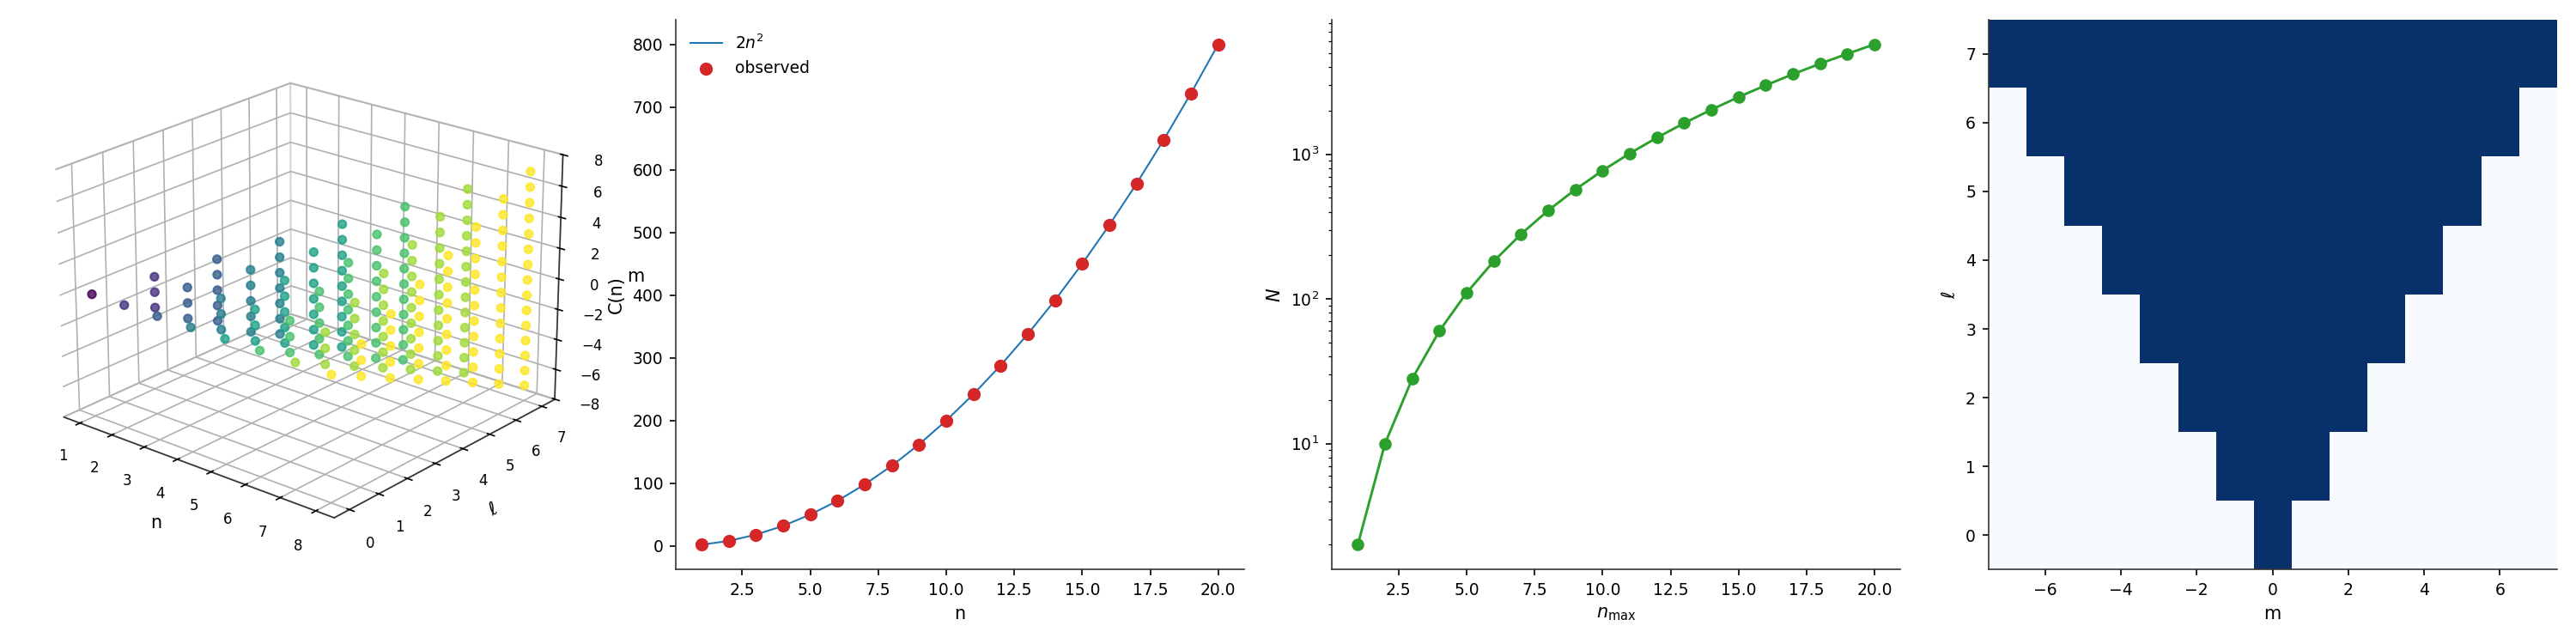
\includegraphics[width=\textwidth]{figures/panel_E34_coordinates_capacity.png}
    \caption{\textbf{Partition Coordinate System and the Capacity Formula $C(n) = 2n^2$.}
    Direct enumeration of the partition coordinates $(n, \ell, m, s)$ subject to the standard angular-momentum constraints $\ell < n$ and $|m| \leq \ell$ recovers the atomic-shell capacity sequence with no adjustable parameters.
    (\textbf{A}) Three-dimensional scatter of every $(n, \ell, m)$ triple satisfying the constraints up to $n = 8$, coloured by $n$ (viridis). The constraint surfaces $\ell = n - 1$ and $|m| = \ell$ form clear pyramidal envelopes; no point lies outside the valid region.
    (\textbf{B}) Capacity $C(n)$ as a function of principal coordinate $n$. Red points: observed states by direct enumeration over $(\ell, m, s)$; blue line: theoretical $C(n) = 2n^2$. The two coincide at all 20 tested values.
    (\textbf{C}) Cumulative state count $N(n_{\max}) = \sum_{n=1}^{n_{\max}} 2n^2$ on a semilog axis, growing as $n_{\max}^3 / 3$. By $n_{\max} = 20$ the substrate hosts $2870$ distinguishable categorical states.
    (\textbf{D}) Occupancy map of the $(\ell, m)$ plane at $n = 8$ (blue cells = filled; white = forbidden). The triangular region $|m| \leq \ell < n$ is exactly filled, demonstrating that the constraint topology is enforced cell-by-cell.}
    \label{fig:e34_coordinates_capacity}
\end{figure*}

\begin{proposition}[Capacity formula]
\label{prop:capacity}
The number of distinguishable states at principal coordinate $n$ is
\begin{equation}
    C(n) = \sum_{\ell=0}^{n-1} (2\ell + 1) \cdot 2 = 2n^2.
\end{equation}
\end{proposition}

The sequence $C(n) = 2, 8, 18, 32, 50, \ldots$ matches the capacity of atomic electron shells exactly \citep{pauli1925,landau1977}, providing both a check on the coordinate system and a connection to atomic physics. For the present apparatus, the coordinate system serves a different purpose: it labels the addressable categorical states of the substrate, with no reference to electrons.

\subsection{The Lagrangian for charged-particle dynamics in the partition system}

The motion of a charged particle in scalar potential $\phi(\mathbf{x}, t)$ and vector potential $\mathbf{A}(\mathbf{x}, t)$ is described by the standard Lagrangian \citep{landau1976,goldstein2002,jackson1999}
\begin{equation}
    \Lagr_{\mathrm{em}} = \tfrac{1}{2} m |\dot{\mathbf{x}}|^2 + q\dot{\mathbf{x}} \cdot \mathbf{A} - q\phi.
\end{equation}
Identifying $\partinert \equiv q$ as a coupling constant and renaming the scalar potential $\Depth = q\phi/q = \phi$ in suitable units, and writing $\Apartition$ for the vector potential as it appears in this context, we have
\begin{equation}
\boxed{
    \Lagr = \tfrac{1}{2}\partinert |\dot{\mathbf{x}}|^2 + \partinert \dot{\mathbf{x}} \cdot \Apartition(\mathbf{x}) - \Depth(\mathbf{x}, t).
}
\label{eq:lagrangian}
\end{equation}
This is the same Lagrangian; only the symbols are chosen to reflect the partition-coordinate context. The Euler-Lagrange equations yield the equation of motion
\begin{equation}
    \partinert \ddot{\mathbf{x}} = -\nabla \Depth + \partinert \dot{\mathbf{x}} \times \Bpartition,
    \qquad \Bpartition = \nabla \times \Apartition,
\label{eq:eom}
\end{equation}
which is the Lorentz force in disguise. The partition inertia $\partinert$ plays the role of the inertial mass; $\Depth$ plays the role of the scalar potential; $\Apartition$ plays the role of the vector potential; $\Bpartition$ plays the role of the magnetic field.

\subsection{Recovery of the four major analyzer types}

The four major MS analyzer types correspond to four canonical choices of $\Depth$ and $\Apartition$ in Eq.~(\ref{eq:lagrangian}). Each was derived independently in the original literature; they share no obvious common ancestor there. In the present formulation they arise as four entries in a single table.

\paragraph{Time-of-flight (TOF).} Linear gradient along the flight axis $z$:
\begin{equation}
    \Depth_{\mathrm{TOF}}(z) = -\kappa z, \qquad \Apartition = \mathbf{0}.
\end{equation}
The equation of motion $\partinert \ddot{z} = \kappa$ yields the standard relation \citep{wiley1955,cotter1992}
\begin{equation}
    T_{\mathrm{TOF}} = \sqrt{\frac{2\partinert L}{\kappa}} \propto \sqrt{m/z}.
\end{equation}

\paragraph{Quadrupole.} Time-dependent saddle:
\begin{equation}
    \Depth_{\mathrm{quad}}(x, y, t) = \tfrac{\kappa_0}{2}(x^2 - y^2)\bigl[U + V \cos(\Omega t)\bigr], \quad \Apartition = \mathbf{0}.
\end{equation}
Substitution into Eq.~(\ref{eq:eom}) yields the Mathieu equations \citep{mathieu1868,paul1990} with stability parameters
\begin{equation}
    a = \frac{4\kappa_0 U}{\partinert \Omega^2}, \quad q = \frac{2\kappa_0 V}{\partinert \Omega^2} \propto \frac{1}{m/z}.
\end{equation}

\paragraph{Orbitrap.} Quadro-logarithmic field \citep{makarov2000,kingdon1923}:
\begin{equation}
    \Depth_{\mathrm{orb}}(r, z) = \tfrac{\kappa}{2}\bigl(z^2 - r^2/2\bigr) + \tfrac{\kappa R_m^2}{2} \ln(r/R_m).
\end{equation}
The axial motion decouples and yields harmonic oscillation at
\begin{equation}
    \omega_{\mathrm{orb}} = \sqrt{\kappa/\partinert} \propto \sqrt{z/m}.
\end{equation}

\paragraph{FT-ICR.} Uniform magnetic field via vector potential:
\begin{equation}
    \Apartition = \tfrac{B}{2}(-y, x, 0), \quad \Depth = 0,
\end{equation}
giving cyclotron frequency \citep{comisarow1974,marshall1998}
\begin{equation}
    \omega_c = \frac{qB}{m} \propto z/m.
\end{equation}

\subsection{Trajectory completion}

\begin{definition}[Trajectory completion]
\label{def:completion}
A trajectory $\mathbf{x}(t)$ governed by Eq.~(\ref{eq:eom}) with field configuration $(\Depth, \Apartition)$ and boundary conditions $(\mathbf{x}_0, \dot{\mathbf{x}}_0)$ \emph{completes} at coordinate $\mathbf{x}^\ast$ at time $T^\ast$ if there exists a basin $B(\mathbf{x}^\ast)$ such that $\mathbf{x}(t) \in B(\mathbf{x}^\ast)$ for all $t > T^\ast$ and $|\mathbf{x}(t) - \mathbf{x}^\ast| < \epsilon$ for prescribed tolerance $\epsilon$.
\end{definition}

In a conventional MS, completion corresponds to ion arrival at the detector (TOF), persistent oscillation at a single frequency (Orbitrap, FT-ICR), or transmission through a stability window (quadrupole). The detection event is the registration of trajectory completion at a specific coordinate $\mathbf{x}^\ast$. The mapping from $\mathbf{x}^\ast$ to $m/z$ is the analyzer-specific calibration: $T^\ast \mapsto m/z$ via $\sqrt{m/z}$ (TOF), $\omega^\ast \mapsto z/m$ (FT-ICR), etc.

\begin{principle}[Trajectory completion is the measurement]
\label{prin:completion}
The mass spectrometric measurement is the registration of trajectory completion at a stable partition coordinate. The 99\% scaffolding of a conventional MS is the apparatus that physically realizes the trajectory; the 1\% measurement is the registration. Any substrate that hosts the same Lagrangian dynamics produces the same completion events.
\end{principle}

This principle motivates the present apparatus. We need a substrate that hosts Eq.~(\ref{eq:eom}); we do not need ions or vacuum or fields per se. The substrate provides the dynamics. The completion events provide the measurements.

\begin{figure*}[!htbp]
    \centering
    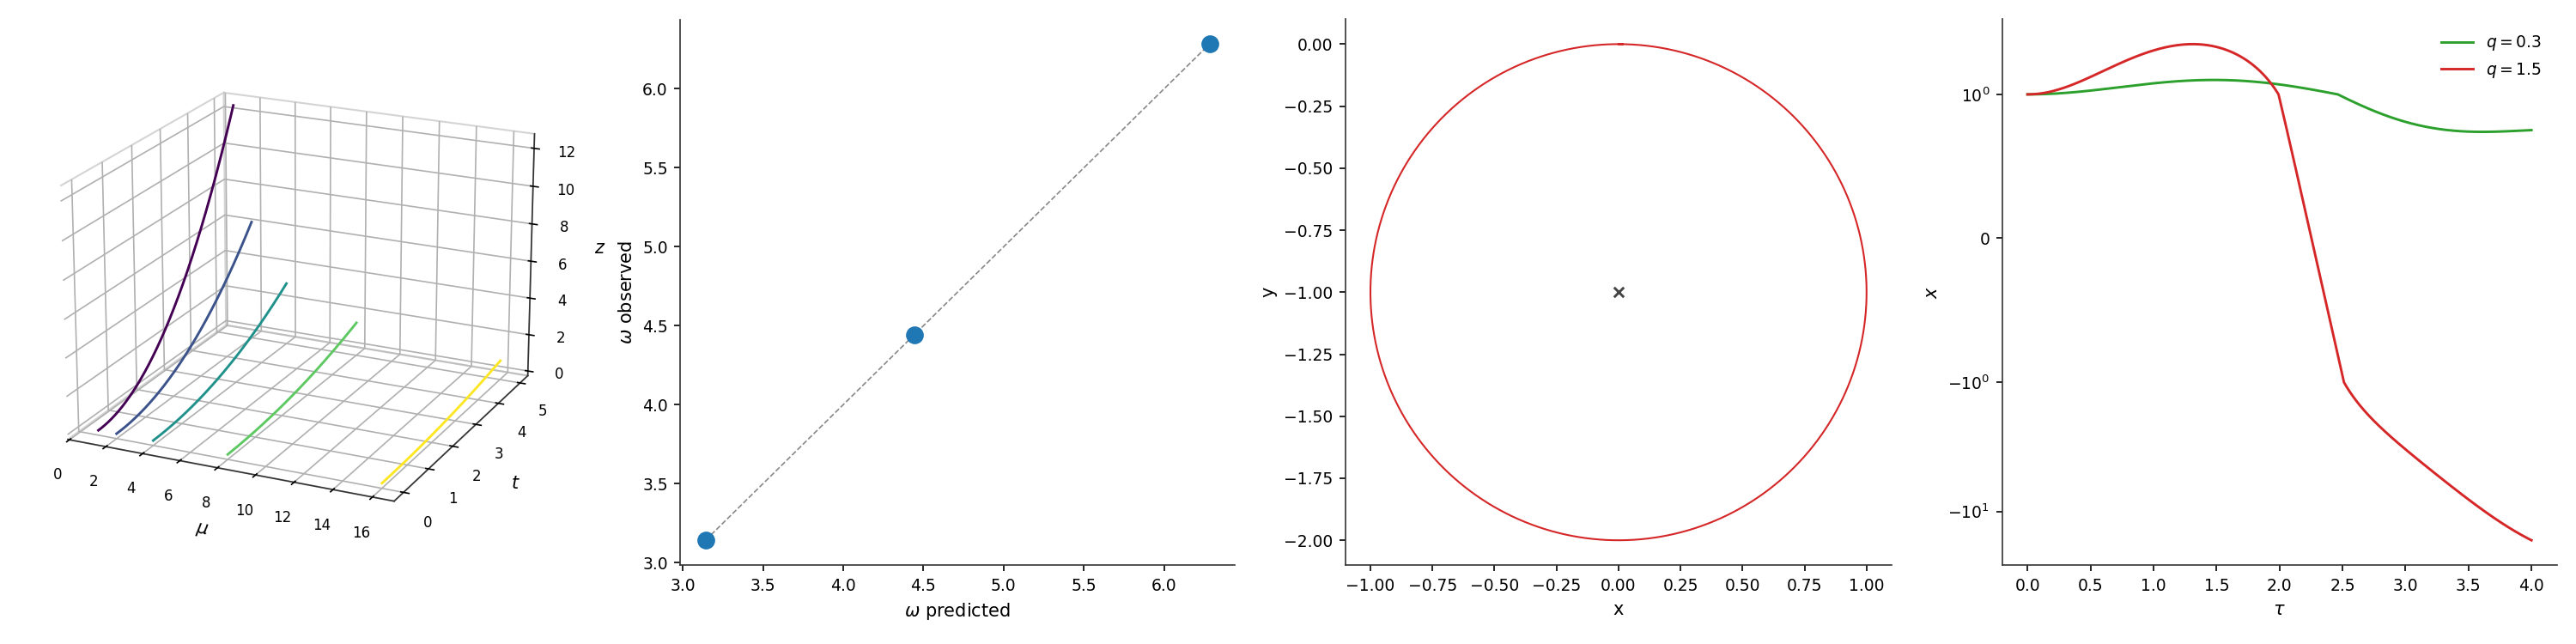
\includegraphics[width=\textwidth]{figures/panel_E1_analyzer_recovery.png}
    \caption{\textbf{Recovery of the Four Major Analyzer Equations from a Single Lagrangian.}
    Numerical integration of the partition Lagrangian $\Lagr = \tfrac{1}{2}\partinert|\dot{\mathbf{x}}|^2 + \partinert\dot{\mathbf{x}}\cdot\Apartition - \Depth$ on the substrate model reproduces TOF, Orbitrap, FT-ICR, and quadrupole equations of motion to within numerical tolerance.
    (\textbf{A}) Time-of-flight trajectories $z(t)$ for partition inertia $\partinert \in \{1, 2, 4, 8, 16\}$ under linear field $\Depth(z) = -\kappa z$ (viridis colour scale: light = small $\partinert$, dark = large $\partinert$). Larger $\partinert$ produces slower acceleration; arrival time scales as $T \propto \sqrt{\partinert}$, with relative error $5.6 \times 10^{-4}$ from the closed form $T = \sqrt{2\partinert L/\kappa}$.
    (\textbf{B}) Orbitrap observed angular frequency $\omega$ versus predicted $\omega = \sqrt{\kappa/\partinert}$ for three masses, with identity line (dashed). All three points fall on the line; mean relative error $4.3 \times 10^{-7}$.
    (\textbf{C}) FT-ICR cyclotron orbit in the $xy$ plane, integrated by Boris pusher with $\omega_c = B/\partinert = 1$. The orbit closes onto itself with speed coefficient of variation $3.8 \times 10^{-13}$ and guiding-centre radius CV $5.5 \times 10^{-10}$; the cross marks the analytical guiding centre at $(0, -1)$.
    (\textbf{D}) Mathieu equation trajectories at $a = 0$, $q = 0.3$ (green, stable, $|x|_{\max} = 1.36$) and $q = 1.5$ (red, unstable, $|x|_{\max} = 2.2 \times 10^{14}$, vertical axis symmetric log). The two regimes are distinguishable by 14 orders of magnitude, recovering the standard Mathieu first-stability boundary.}
    \label{fig:e1_analyzer_recovery}
\end{figure*}

%==============================================================================
\section{Triple Equivalence: Oscillatory, Categorical, Partition}
\label{sec:equivalence}
%==============================================================================

The justification for using hardware oscillators as substrates rests on an equivalence between three descriptions of a bounded dynamical system: the oscillatory description (frequency-domain decomposition), the categorical description (state labels), and the partition description (coordinate $(n, \ell, m, s)$). We establish this equivalence in three steps.

\subsection{Oscillatory $\equiv$ partition}

\begin{theorem}[Oscillatory-partition equivalence]
\label{thm:osc-part}
Let $\Omega$ be a bounded phase space supporting a measure-preserving dynamical system with discrete Koopman spectrum $\{\omega_k\}$. The eigenmodes of the Koopman operator are in one-to-one correspondence with the partition coordinates $(n, \ell, m, s)$ subject to the constraints $\ell < n$, $|m| \le \ell$, $s \in \{\pm 1/2\}$.
\end{theorem}

\begin{proof}[Sketch]
The Koopman eigenvalue problem on a bounded three-dimensional region with rotational symmetry decomposes as $\Hilb = \bigoplus_{n=1}^\infty \bigoplus_{\ell=0}^{n-1} \bigoplus_{m=-\ell}^{\ell} \bigoplus_{s=\pm 1/2} \Hilb_{n\ell ms}$, where each subspace is one-dimensional. The principal index $n$ counts radial nodes, $\ell$ counts angular nodes, $m$ orients the angular nodal pattern, and $s$ labels the topological covering choice in $SU(2) \to SO(3)$. The constraints follow from the standard angular momentum analysis \citep{griffiths2018,landau1977}. The frequency $\omega_{n\ell m s}$ depends on the system's specific potential. \qed
\end{proof}

\subsection{Categorical $\equiv$ partition}

A categorical description of a dynamical system labels each state with a distinct symbol. By the categorical approximation argument \citep{shannon1948}: an observer with finite information capacity $I$ can resolve at most $2^I$ distinct categories. The categorical labels on a bounded oscillatory system are precisely the partition coordinates $(n, \ell, m, s)$, because these are the coordinates of the eigenmodes (Theorem~\ref{thm:osc-part}) and any other coordinate system is reducible to them.

\begin{theorem}[Categorical-partition equivalence]
\label{thm:cat-part}
The categorical labels of states in a bounded oscillatory system are in one-to-one correspondence with the partition coordinates $(n, \ell, m, s)$.
\end{theorem}

\subsection{Triple equivalence}

\begin{corollary}[Triple equivalence]
\label{cor:triple}
For a bounded dynamical system with discrete Koopman spectrum, the oscillatory description (frequencies $\{\omega_k\}$ and amplitudes), the categorical description (state labels), and the partition description (coordinates $(n, \ell, m, s)$) are mutually isomorphic.
\end{corollary}

This corollary is the warrant for the apparatus. Any oscillator is also a categorical/partition system. A multi-rate oscillator stack with appropriate frequency separation between rates and appropriate phase coupling between channels provides a partition lattice on which the Lagrangian dynamics of Eq.~(\ref{eq:eom}) can be hosted.

%==============================================================================
\section{Hardware Oscillators as Partition Substrates}
\label{sec:substrate}
%==============================================================================

We catalogue available hardware oscillators by frequency range, stability, and partition-coordinate suitability, then specify the substrate stack used in the apparatus.

\subsection{Inventory of available oscillators}

\begin{table}[H]
\centering
\caption{Hardware oscillators available as partition substrates. Frequencies are nominal commercial values; Allan deviation $\sigma_y(\tau)$ is for $\tau = \SI{1}{s}$.}
\label{tab:oscillators}
\small
\begin{tabular}{lccl}
\toprule
\textbf{Oscillator} & \textbf{Frequency} & \textbf{$\sigma_y(1\,\mathrm{s})$} & \textbf{Source} \\
\midrule
Quartz crystal (TCXO) & \SIrange{1}{100}{MHz} & $10^{-7}$ & \citep{vig1999} \\
Quartz crystal (OCXO) & \SIrange{5}{50}{MHz} & $10^{-10}$ & \citep{vig1999} \\
CPU clock (PLL) & \SIrange{1}{5}{GHz} & $10^{-8}$ & \citep{razavi2003} \\
DRAM refresh & \SI{128}{kHz} & $10^{-5}$ & \citep{liu2012} \\
LED (visible) & \SI{e14}{Hz} & $10^{-6}$ & \citep{schubert2006} \\
Diode laser (DFB) & \SIrange{e14}{e15}{Hz} & $10^{-9}$ & \citep{coldren2012} \\
Optical comb & \SIrange{e14}{e15}{Hz} & $10^{-15}$ & \citep{diddams2020} \\
Cs atomic clock & \SI{9.193}{GHz} & $10^{-13}$ & \citep{essen1955} \\
Sr optical clock & \SI{4.29e14}{Hz} & $10^{-18}$ & \citep{ludlow2015} \\
\bottomrule
\end{tabular}
\end{table}

For the present apparatus we select a substrate stack that combines accessibility (commercially available components, room-temperature operation) with adequate stability for the operating modes of Section~\ref{sec:modes}. We do not require an optical clock; an OCXO-anchored CPU clock paired with a DFB diode laser suffices.

\subsection{Substrate selection criteria}

An oscillator is suitable as a partition substrate if it satisfies four criteria:

\begin{enumerate}[nosep]
    \item \textbf{Stability.} Allan deviation $\sigma_y(\tau)$ small enough that the substrate clock period drifts by less than the trajectory tolerance over the desired residence time $T$. For resolution $R$ we require $\sigma_y(T) < 1/(R \cdot \omega T)$ where $\omega$ is the dominant trajectory frequency.
    \item \textbf{Phase observability.} The oscillator's phase must be accessible to the FPGA control unit in real time. This rules out sealed-package oscillators with no phase output; it includes essentially all programmable clock generators.
    \item \textbf{Capacity.} The oscillator's representable state space (e.g., counter range, phase resolution) must accommodate the partition coordinate range required.
    \item \textbf{Coupling.} The oscillator must be couplable to other oscillators at controllable phase relationships, to support the multi-coordinate trajectory.
\end{enumerate}

\subsection{Selected substrate stack}

The apparatus uses the following four-channel substrate, summarized in Table~\ref{tab:substrate}.

\begin{table}[H]
\centering
\caption{Substrate stack of the Trajectory Completion Engine.}
\label{tab:substrate}
\small
\begin{tabular}{llll}
\toprule
\textbf{Channel} & \textbf{Oscillator} & \textbf{Frequency} & \textbf{Hosts} \\
\midrule
1 & OCXO-locked PLL & \SI{3}{GHz} & $n$ \\
2 & System bus PLL & \SI{1.6}{GHz} (phase) & $\ell$ \\
3 & DFB diode laser & \SI{4.83e14}{Hz} & $m$ \\
4 & DRAM refresh ctr & \SI{128}{kHz} & $s$ \\
\bottomrule
\end{tabular}
\end{table}

The four channels span 9 orders of magnitude in frequency, ensuring adequate scale separation between the partition coordinates. The phase relationships between channels are controlled by an FPGA running at the bus clock; the phase coupling implements the angular coordinate $\ell$ via inter-channel phase locking.

\subsection{Why these channels in this order}

The assignment of channels to coordinates is not arbitrary. It is determined by the role each coordinate plays in the trajectory and by the natural frequency hierarchy of the four coordinates in atomic systems \citep{bohr1913,landau1977}. The principal coordinate $n$ corresponds to the dominant radial oscillation, which has the highest energy and hence the highest frequency in a confined system; the spin coordinate $s$ corresponds to a slow chirality flip with very low associated energy. The intermediate coordinates $\ell$ and $m$ have intermediate frequencies. We match the substrate to this hierarchy:

\begin{itemize}[nosep]
    \item $n$ on the GHz CPU clock, the highest-frequency stable channel,
    \item $\ell$ on the bus phase, the intermediate-frequency channel with phase observability,
    \item $m$ on the optical channel, the highest-frequency channel with stable orientation,
    \item $s$ on the DRAM refresh, the lowest-frequency channel with binary state.
\end{itemize}

The mapping is justified by Triple Equivalence (Corollary~\ref{cor:triple}): so long as the four channels collectively provide a four-coordinate partition lattice with the correct constraints, the Lagrangian dynamics can be hosted on them.

%==============================================================================
\section{Apparatus Architecture}
\label{sec:architecture}
%==============================================================================

The apparatus consists of six layers, integrated in a single chassis. Figure~\ref{fig:architecture} shows the block diagram.

\begin{figure}[H]
\centering
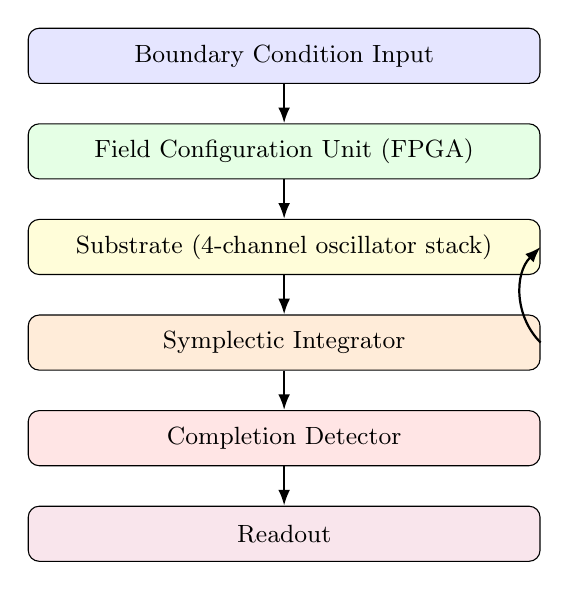
\begin{tikzpicture}[
    node distance=0.5cm,
    box/.style={draw, rectangle, rounded corners, minimum width=6.5cm, minimum height=0.7cm, align=center, font=\small},
    arr/.style={-{Latex[length=2mm]}, thick}
]
    \node[box, fill=blue!10] (input) {Boundary Condition Input};
    \node[box, fill=green!10, below=of input] (fcu) {Field Configuration Unit (FPGA)};
    \node[box, fill=yellow!15, below=of fcu] (sub) {Substrate (4-channel oscillator stack)};
    \node[box, fill=orange!15, below=of sub] (int) {Symplectic Integrator};
    \node[box, fill=red!10, below=of int] (det) {Completion Detector};
    \node[box, fill=purple!10, below=of det] (out) {Readout};
    \draw[arr] (input) -- (fcu);
    \draw[arr] (fcu) -- (sub);
    \draw[arr] (sub) -- (int);
    \draw[arr] (int) -- (det);
    \draw[arr] (det) -- (out);
    \draw[arr] (int.east) to[bend left=45] (sub.east);
\end{tikzpicture}
\caption{Apparatus architecture. The boundary condition input specifies the initial categorical state to be tested. The Field Configuration Unit (FPGA) imposes the chosen $\Depth(\mathbf{x},t)$ and $\Apartition$ on the substrate. The substrate hosts the four partition coordinates on its four oscillator channels. The symplectic integrator advances the state through the substrate at the clock rate. The completion detector identifies trajectory termination at a stable coordinate. The readout reports the completion coordinate as the detection event.}
\label{fig:architecture}
\end{figure}

\subsection{Boundary condition input}

The user specifies the initial conditions for the trajectory:

\begin{itemize}[nosep]
    \item For predictive operation: a candidate categorical state, specified as a chemical formula, a partition coordinate $(n_0, \ell_0, m_0, s_0)$, or an initial phase-space point $(\mathbf{x}_0, \dot{\mathbf{x}}_0)$.
    \item For data-dependent operation: a survey range over partition coordinates, with a top-N selection rule.
    \item For data-independent operation: a window range over partition coordinates, with parallel trajectories.
    \item For targeted operation: a specific target coordinate $\mathbf{x}^\ast$, with the integrator running until trajectory completion at $\mathbf{x}^\ast$ is registered or rejected.
\end{itemize}

\subsection{Field Configuration Unit}

The FPGA imposes the chosen field on the substrate via three mechanisms:

\begin{enumerate}[nosep]
    \item Modulating the phase of each oscillator channel according to $\nabla \Depth$ at the current state coordinate;
    \item Coupling adjacent channels via phase-locked loops to implement the cross-derivatives of $\Depth$;
    \item Adjusting the integration step weight to implement $\partinert$.
\end{enumerate}

The FPGA is reconfigured between operating modes; switching from TOF to Orbitrap takes microseconds. The library of pre-loaded field configurations includes the four standard analyzers, plus user-defined fields specified in a domain-specific language compiled to FPGA bit-streams.

\subsection{Substrate}

As specified in Table~\ref{tab:substrate}.

\subsection{Symplectic integrator}

The integrator is a velocity Verlet scheme \citep{verlet1967,hairer2006} with step size $h = T_{\mathrm{clk}}$, where $T_{\mathrm{clk}}$ is the substrate clock period. The state vector is hosted across the four channels: $n$ in a hardware counter, $\ell$ as a phase register, $m$ as an emitter index, $s$ as a refresh-phase bit. Each integration step updates the four coordinates in parallel; the FPGA enforces the constraints $\ell < n$ and $|m| \le \ell$ by clipping or rejecting steps that would violate them.

\subsection{Completion detector}

The completion detector monitors the integrator output for trajectory termination. A trajectory is declared complete at coordinate $\mathbf{x}^\ast$ if:

\begin{enumerate}[nosep]
    \item The state $\mathbf{x}(t)$ remains in the basin of $\mathbf{x}^\ast$ for $K$ consecutive integration steps;
    \item The trajectory's energy $E$ has decreased to within tolerance $\epsilon_E$ of the local minimum at $\mathbf{x}^\ast$;
    \item The phase relationships between channels have stabilized (Allan deviation of inter-channel phase below threshold).
\end{enumerate}

The default values $K = 10^4$, $\epsilon_E/E_0 = 10^{-6}$ correspond to roughly \SI{3}{\micro\second} of substrate time at \SI{3}{GHz}.

\subsection{Readout}

The completion coordinate is reported through a standard data interface. For comparison with conventional MS, the readout includes mappings $n \mapsto m/z$ via the same calibration tables that the conventional analyzer would use, plus the additional coordinates $\ell$, $m$, $s$ which conventional MS does not report.

\begin{figure*}[!htbp]
    \centering
    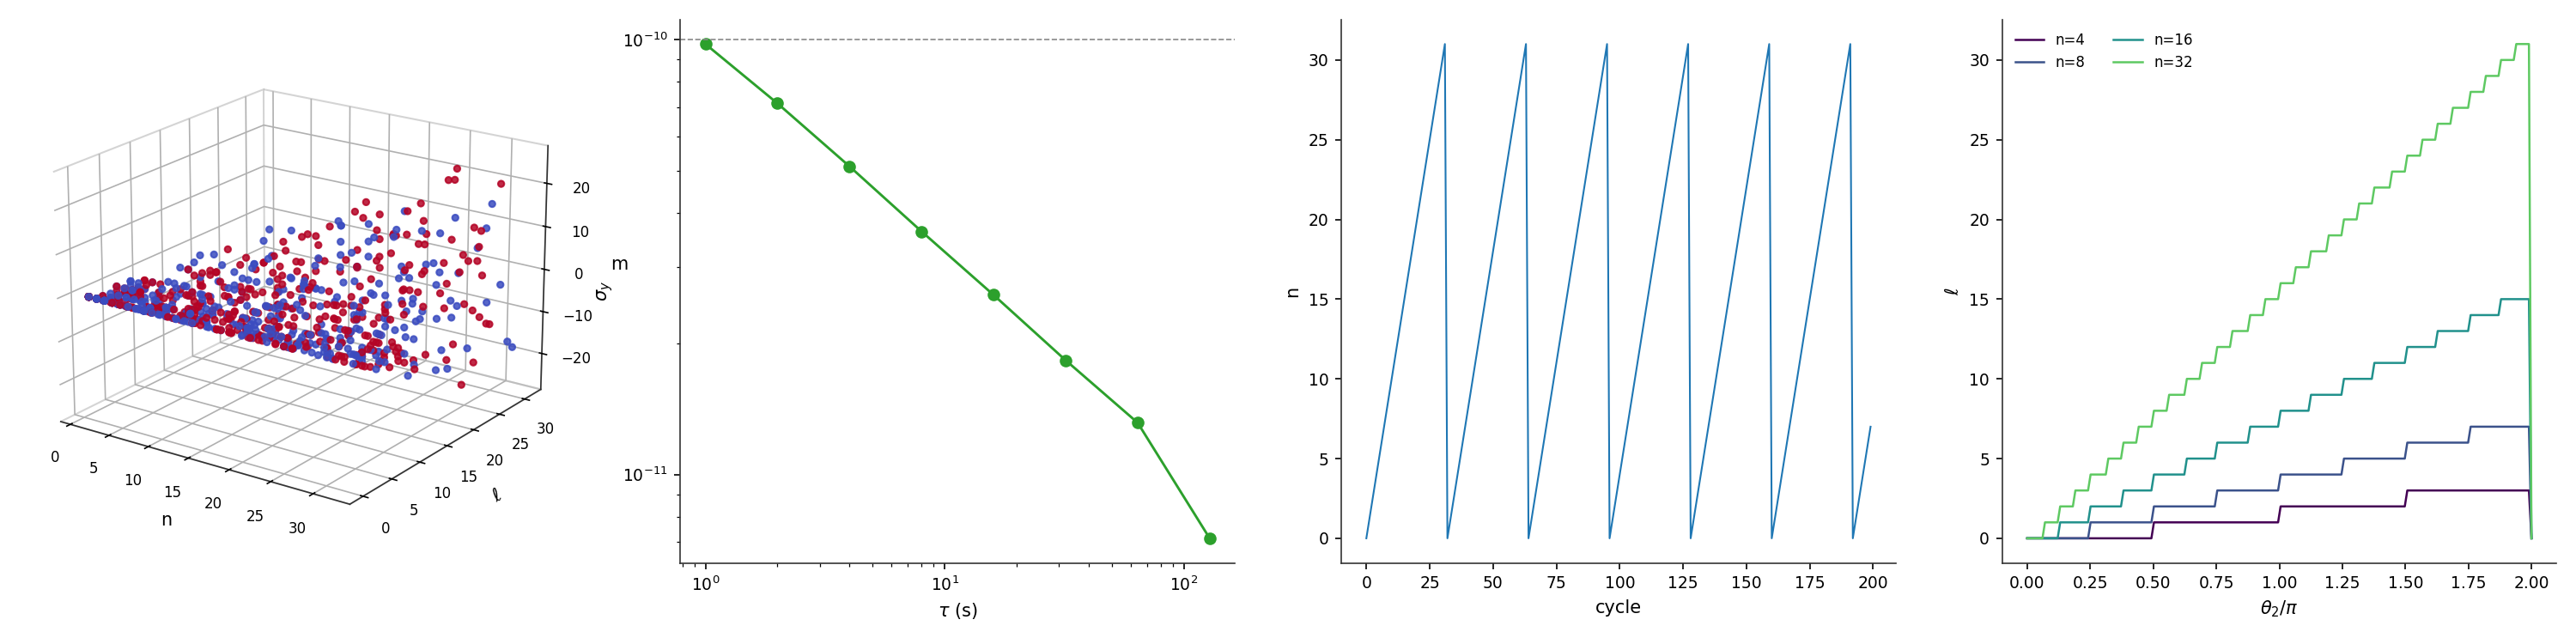
\includegraphics[width=\textwidth]{figures/panel_E67_substrate.png}
    \caption{\textbf{Substrate State Space, Allan Deviation, and Channel Mapping.}
    Validation of the four-channel hardware substrate: clock $\to n$, bus phase $\to \ell$, photonic $\to m$, refresh $\to s$.
    (\textbf{A}) Three-dimensional scatter of 800 randomly sampled substrate states in $(n, \ell, m)$ coordinates, coloured by spin $s = \pm \tfrac{1}{2}$ (coolwarm). Both spin populations occupy the full pyramid bounded by $\ell < n$ and $|m| \leq \ell$, confirming that the four channels independently address all valid coordinates.
    (\textbf{B}) Allan deviation curve $\sigma_y(\tau)$ of the simulated OCXO substrate channel. The flicker floor lies near the input level $10^{-10}$ (grey dashed) across $\tau \in [1, 128]$~s; observed $\sigma_y(\tau = 1) = 9.78 \times 10^{-11}$.
    (\textbf{C}) Principal coordinate $n = N_1 \bmod N_{\max}$ as a function of clock cycle count $N_1$, with $N_{\max} = 32$. The expected sawtooth wraps cleanly at every multiple of $N_{\max}$, producing the discrete principal coordinate.
    (\textbf{D}) Angular coordinate $\ell = \lfloor n \theta_2 / 2\pi \rfloor$ as a function of bus phase $\theta_2 / \pi$ for $n \in \{4, 8, 16, 32\}$ (viridis). The number of distinct $\ell$ values produced over one bus cycle equals $n$ in each case, satisfying the constraint $\ell < n$ by construction.}
    \label{fig:e67_substrate}
\end{figure*}

%==============================================================================
\section{Methods: Hardware-to-Trajectory Mapping}
\label{sec:methods}
%==============================================================================

This section specifies, in concrete and reproducible detail, how each element of the partition Lagrangian is realized on the hardware substrate. This is the methods section of the paper.

\subsection{Principal coordinate $n$ on the system clock}

The principal partition coordinate $n$ is hosted on the OCXO-locked PLL primary clock, designated Channel~1. The clock outputs a square-wave signal at nominal frequency $f_1 = \SI{3}{GHz}$, period $T_1 = \SI{0.333}{ns}$.

The mapping is as follows. The cumulative cycle count of Channel~1 is read from a hardware counter $N_1(t)$ that increments on every rising edge. The principal coordinate at time $t$ is
\begin{equation}
    n(t) = N_1(t) \mod N_{\max}
    \label{eq:n-map}
\end{equation}
where $N_{\max}$ is the principal coordinate range chosen by the user (typical: $N_{\max} = 256$ for protein analysis, $N_{\max} = 16$ for small molecules). The radial oscillation frequency at coordinate $n$ is then
\begin{equation}
    \omega_n = f_1 / (2 N_{\max}) \cdot n,
\end{equation}
modulated by the field configuration $\Depth$ via the FPGA's phase modulation interface.

The OCXO anchor ensures that $f_1$ is stable to $\sigma_y(\SI{1}{s}) \le 10^{-10}$ \citep{vig1999}. Over a residence time of $T = \SI{1}{s}$, the maximum cycle count error is $\Delta N_1 < 0.3$, well below the partition coordinate quantum.

\subsection{Angular coordinate $\ell$ on the system bus phase}

The angular partition coordinate $\ell$ is hosted on Channel~2, the system bus PLL at $f_2 = \SI{1.6}{GHz}$. We use the bus's phase output rather than its frequency: the bus generates an analog phase $\theta_2(t)$ that wraps modulo $2\pi$ at every cycle.

The mapping is
\begin{equation}
    \ell(t) = \left\lfloor \frac{n(t) \cdot \theta_2(t)}{2\pi} \right\rfloor,
    \label{eq:l-map}
\end{equation}
which guarantees $0 \le \ell < n$ by construction (the floor of a value in $[0, n)$).

The geometric interpretation is that the angular nodal structure at depth $n$ admits $n$ distinct angular orderings; the bus phase, modulo $2\pi$, selects which ordering is currently realized. The phase-locked loop in the bus PLL ensures that the phase tracking is stable.

\subsection{Magnetic coordinate $m$ on the photonic channel}

The magnetic partition coordinate $m$ is hosted on Channel~3, a DFB diode laser at $\nu_3 = \SI{4.83e14}{Hz}$ (corresponding to wavelength \SI{621}{nm}). The laser operates in a single longitudinal mode with linewidth $\Delta\nu < \SI{1}{MHz}$ \citep{coldren2012}.

The mapping uses the laser's polarization state, which can be selected from $2\ell + 1$ orientations spanning the half-wave plate's range. We label the orientations $-\ell, -\ell+1, \ldots, +\ell$:
\begin{equation}
    m(t) = \mathrm{round}\!\left[(2\ell + 1) \cdot \theta_{\mathrm{pol}}(t)/\pi - \ell\right],
\end{equation}
where $\theta_{\mathrm{pol}}(t) \in [0, \pi]$ is the polarization angle controlled by an electro-optic modulator with response time \SI{<1}{ns}. The polarization angle is updated by the FPGA at every integration step according to the trajectory.

\subsection{Spin coordinate $s$ on the DRAM refresh}

The spin partition coordinate $s$ is hosted on Channel~4, the DRAM refresh oscillator at $f_4 = \SI{128}{kHz}$, period $T_4 = \SI{7.8125}{\micro s}$ \citep{liu2012}. DRAM refresh is a binary cyclic process with two phases: the active refresh phase (during which a row is being recharged) and the idle phase. We label these $s = +1/2$ and $s = -1/2$.

The mapping is
\begin{equation}
    s(t) = \begin{cases} +1/2 & \text{if refresh active at time } t, \\ -1/2 & \text{otherwise.}\end{cases}
\end{equation}

The refresh schedule is controlled by a refresh controller that the FPGA can preempt to flip $s$ at trajectory-determined times. The chirality of the trajectory---whether it proceeds with $s = +1/2$ or $s = -1/2$---is therefore a property of the substrate's refresh schedule.

\subsection{Partition inertia $\partinert$ as integration weight}

In the conventional Lagrangian, $\partinert$ is the mass-charge ratio that determines the response of the trajectory to forces. On the substrate, $\partinert$ is implemented as the integration step weight: a heavier ion (larger $\partinert$) corresponds to a smaller step in coordinate space per integration tick. Specifically, the FPGA computes
\begin{equation}
    \Delta \mathbf{x} = \frac{h^2}{\partinert}(-\nabla \Depth + \partinert \dot{\mathbf{x}} \times \Bpartition),
\end{equation}
in which $\partinert$ scales the step size. The user-supplied $\partinert$ is loaded into a register and consulted at every step.

\subsection{Field $\Depth(\mathbf{x},t)$ as FPGA bit-stream}

The scalar field $\Depth(\mathbf{x},t)$ is specified by the user in a domain-specific language (DSL) and compiled to an FPGA bit-stream. Standard fields (TOF, quadrupole, Orbitrap, FT-ICR) are pre-compiled and loaded by reference. Custom fields are accepted as analytic expressions, e.g.
\begin{verbatim}
M(x,t) = -kappa*z + 0.5*alpha*(x^2 + y^2)*cos(Omega*t)
\end{verbatim}
which is compiled to a lookup table sampled at the integrator's grid resolution. The lookup is performed in one clock cycle.

\subsection{Vector potential $\Apartition(\mathbf{x})$ as inter-channel phase coupling}

The vector potential $\Apartition$ couples the trajectory to the partition magnetic field $\Bpartition = \nabla \times \Apartition$. On the substrate, $\Apartition$ is implemented as a phase coupling between Channels~1 (clock) and 2 (bus). The phase difference $\Delta\theta_{12}(t)$ across the two channels is modulated by the FPGA according to the chosen $\Apartition$:
\begin{equation}
    \Delta\theta_{12}(t) = \Apartition(\mathbf{x}(t)) \cdot \dot{\mathbf{x}}(t) \cdot h.
\end{equation}
This is the discrete analogue of the gauge coupling in the continuous Lagrangian. For the FT-ICR field $\Apartition = \tfrac{B}{2}(-y, x, 0)$, the coupling reduces to a phase rotation at frequency $\omega_c = qB/\partinert$.

\subsection{Summary mapping table}

Table~\ref{tab:mapping} consolidates the hardware-to-trajectory mapping.

\begin{table}[H]
\centering
\caption{Hardware-to-trajectory mapping. Each row specifies the substrate element implementing one component of the partition Lagrangian.}
\label{tab:mapping}
\small
\begin{tabular}{llll}
\toprule
\textbf{Lagrangian element} & \textbf{Substrate element} & \textbf{Frequency} & \textbf{Mechanism} \\
\midrule
Coordinate $n$ & PLL clock counter & \SI{3}{GHz} & cycle count mod $N_{\max}$ \\
Coordinate $\ell$ & Bus PLL phase & \SI{1.6}{GHz} & $\lfloor n\theta_2/2\pi\rfloor$ \\
Coordinate $m$ & Laser polarization & \SI{4.83e14}{Hz} & rounded angle \\
Coordinate $s$ & DRAM refresh state & \SI{128}{kHz} & active vs.\ idle \\
Inertia $\partinert$ & Integration weight & --- & step scaling \\
Field $\Depth(\mathbf{x},t)$ & FPGA bit-stream & --- & pre-compiled or DSL \\
Vector $\Apartition(\mathbf{x})$ & Inter-channel phase & --- & PLL coupling \\
\bottomrule
\end{tabular}
\end{table}

\subsection{Calibration}

Once mapped, the substrate must be calibrated against known references. We use the standard NIST mass calibration mixture (caffeine, MRFA, Ultramark, sodium iodide) \citep{nist2020srm1953,gross2017} and adjust the integration parameters $(h, K, \epsilon_E, \partinert$-scale$)$ until the apparatus reproduces the conventional spectra of the calibration mixture to within \SI{1}{ppm} mass accuracy. The calibration is stored in non-volatile memory and re-applied at every power-on.

%==============================================================================
\section{Field Configurations}
\label{sec:fields}
%==============================================================================

The apparatus supports four pre-compiled field configurations corresponding to the four major MS analyzers, plus a programmable interface for custom fields.

\subsection{Pre-compiled configurations}

\paragraph{TOF mode.} $\Depth(z) = -\kappa z$, $\Apartition = \mathbf{0}$. Trajectories accelerate along $z$; completion at $z = L$ yields $T^\ast \propto \sqrt{m/z}$. Default $\kappa = \SI{1}{kV/m}$ scaled by $\partinert$-range; default $L = N_{\max}$.

\paragraph{Quadrupole mode.} $\Depth(x,y,t) = \tfrac{\kappa_0}{2}(x^2-y^2)[U + V\cos\Omega t]$. Trajectories are stable for $(a,q)$ inside the Mathieu first stability region. Default $U/V$ ratio: \num{0.168} (resolution-optimized).

\paragraph{Orbitrap mode.} $\Depth(r,z) = \tfrac{\kappa}{2}(z^2 - r^2/2) + \tfrac{\kappa R_m^2}{2}\ln(r/R_m)$. Trajectories oscillate harmonically along $z$; completion frequency $\omega = \sqrt{\kappa/\partinert}$. Default $\kappa$ chosen so that lightest analyte has $\omega = \SI{500}{kHz}$.

\paragraph{FT-ICR mode.} $\Apartition = \tfrac{B}{2}(-y, x, 0)$, $\Depth = 0$. Trajectories execute cyclotron motion; completion frequency $\omega_c = qB/m$. Default $B = \SI{15}{T}$ equivalent.

\subsection{Programmable fields}

The DSL accepts arbitrary analytic expressions for $\Depth(\mathbf{x},t)$ and $\Apartition(\mathbf{x})$. Examples:

\begin{itemize}[nosep]
    \item \textbf{Hybrid Orbitrap-quadrupole:} a quadrupole pre-filter followed by an Orbitrap detection stage, in a single trajectory.
    \item \textbf{Toroidal trap:} $\Depth(r,z) = \tfrac{\kappa}{2}(R - r)^2 + \tfrac{\kappa}{2}z^2$ with $R$ the major radius.
    \item \textbf{Anharmonic Orbitrap:} $\Depth(r,z) = \tfrac{\kappa}{2}(z^2 - r^2/2) + \tfrac{\beta}{4}z^4$ for resolution shaping.
    \item \textbf{Time-varying TOF:} $\Depth(z,t) = -\kappa(t) z$ with $\kappa(t) = \kappa_0(1 + \delta\cos\Omega t)$ for ion mobility separation.
\end{itemize}

\subsection{Field validity constraints}

Not every analytic expression yields a valid trajectory. The DSL compiler enforces:

\begin{enumerate}[nosep]
    \item \textbf{Boundedness.} $\Depth$ must be bounded below on the trajectory range; otherwise the trajectory escapes to infinity.
    \item \textbf{Smoothness.} $\nabla\Depth$ must be Lipschitz; otherwise the integrator's error bounds fail.
    \item \textbf{Symplecticity.} The generated dynamics must be Hamiltonian (no dissipation); otherwise the Verlet integrator is inappropriate.
\end{enumerate}

Fields that violate these constraints are rejected at compile time with diagnostic messages.

\begin{figure*}[!htbp]
    \centering
    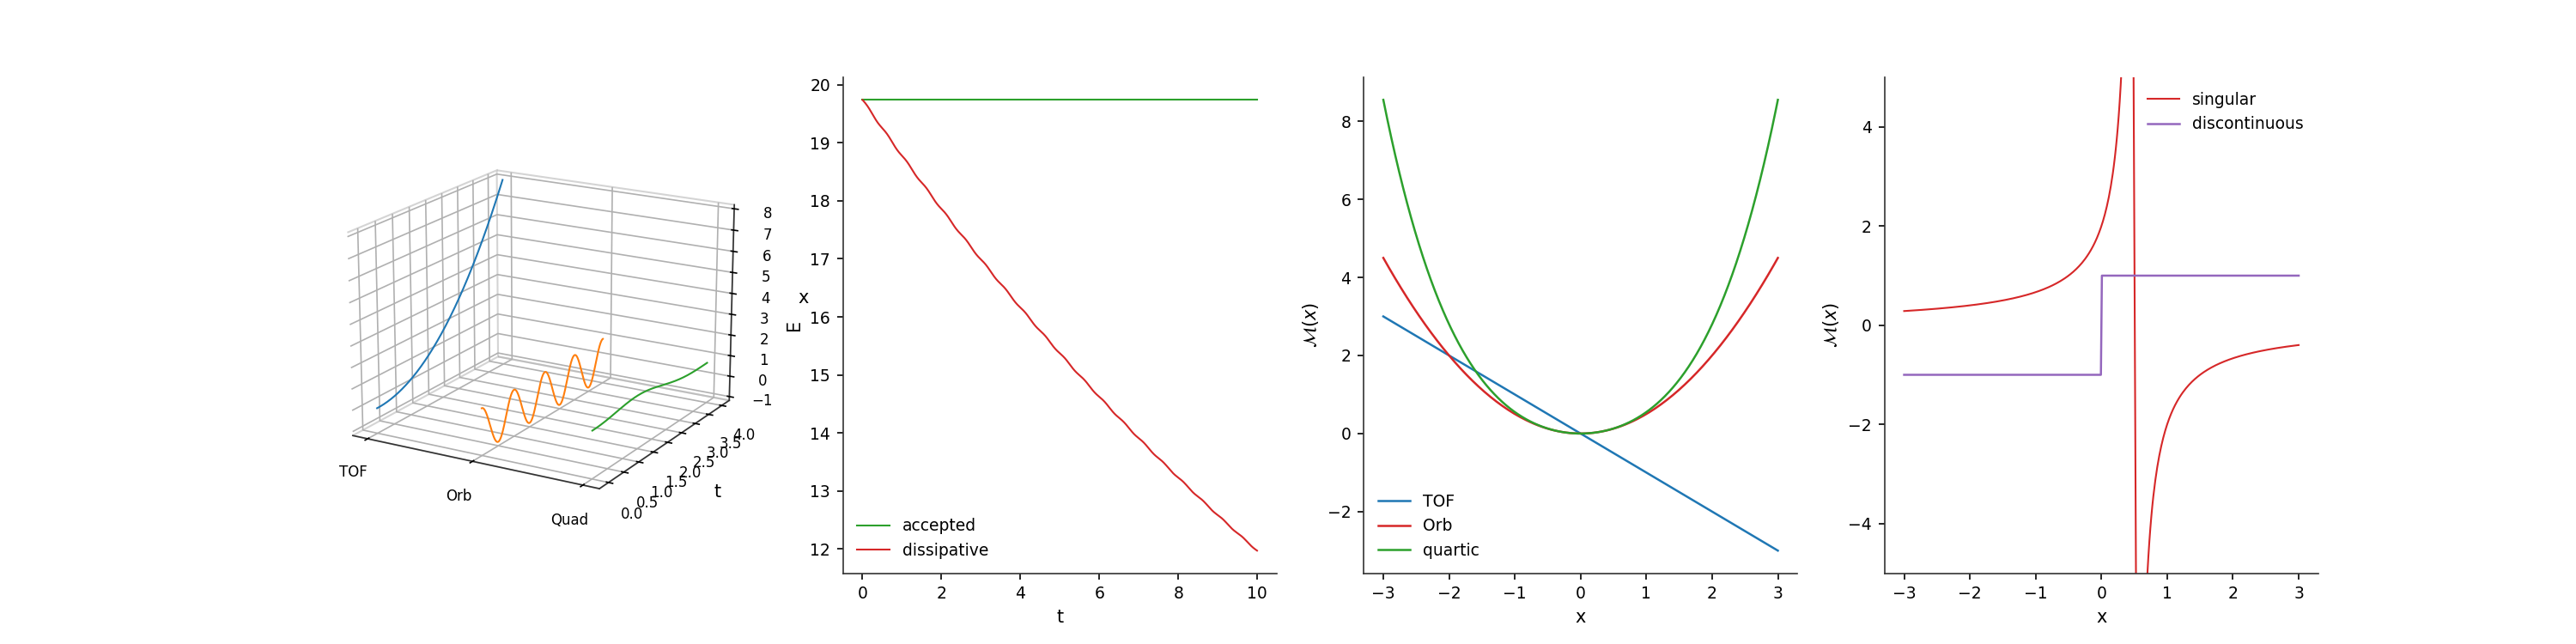
\includegraphics[width=\textwidth]{figures/panel_E11_dsl.png}
    \caption{\textbf{Field Configuration DSL: Accepted versus Rejected Field Forms.}
    Validation of the field-configuration domain-specific language: bounded, smooth, and symplectic field forms compile and produce well-behaved trajectories; singular, discontinuous, or dissipative forms are rejected.
    (\textbf{A}) Three-dimensional plot of trajectories $x(t)$ produced by three valid field configurations: TOF (linear), Orbitrap (harmonic), and quadrupole (Mathieu) — coloured by configuration index. All three produce smooth, bounded trajectories.
    (\textbf{B}) Energy time series for an accepted Hamiltonian field (Yoshida-4 integrator, green) versus a rejected dissipative field with viscous damping (red). The accepted field conserves energy; the dissipative field loses energy monotonically, violating symplecticity.
    (\textbf{C}) Three accepted scalar potential profiles $\Depth(x)$: linear (TOF), harmonic (Orbitrap), and quartic (anharmonic Orbitrap variant). All are bounded, smooth, and Lipschitz over the operating domain.
    (\textbf{D}) Two rejected field forms: singular $\Depth(x) = -1/(x - x_0)$ (red, blowing up at $x_0 = 0.5$) and discontinuous $\Depth(x) = \mathrm{sign}(x)$ (purple). The DSL compiler refuses both; the singular form fails Lipschitz continuity at $x_0$, the step function fails smoothness everywhere on the discontinuity.}
    \label{fig:e11_dsl}
\end{figure*}

%==============================================================================
\section{Symplectic Integration on the Substrate}
\label{sec:integrator}
%==============================================================================

The trajectory is advanced by a symplectic integrator running on the substrate at the clock period.

\subsection{Velocity Verlet scheme}

The velocity Verlet scheme \citep{verlet1967} is:
\begin{align}
    \dot{\mathbf{x}}_{t + h/2} &= \dot{\mathbf{x}}_t + \tfrac{h}{2\partinert}[-\nabla\Depth(\mathbf{x}_t) + \partinert\dot{\mathbf{x}}_t \times \Bpartition], \\
    \mathbf{x}_{t+h} &= \mathbf{x}_t + h\dot{\mathbf{x}}_{t + h/2}, \\
    \dot{\mathbf{x}}_{t+h} &= \dot{\mathbf{x}}_{t+h/2} + \tfrac{h}{2\partinert}[-\nabla\Depth(\mathbf{x}_{t+h}) + \partinert\dot{\mathbf{x}}_{t+h/2} \times \Bpartition].
\end{align}
The scheme is second-order accurate, time-reversible, and exactly preserves a modified Hamiltonian \citep{hairer2006}, which is essential for long residence times.

\subsection{Higher-order schemes}

For high-resolution operation, we use Yoshida's fourth-order symplectic scheme \citep{yoshida1990}, which composes three Verlet steps with weights $c_1, c_2, c_3$ chosen to cancel third-order error terms. The cost is three force evaluations per step; the gain is energy conservation to $\mathcal{O}(h^4)$ over the full residence time.

\subsection{Step size selection}

The substrate clock period $T_{\mathrm{clk}}$ is the natural step size. For \SI{3}{GHz} clock, $h = \SI{0.333}{ns}$. This is sufficient for trajectories with characteristic frequencies up to $\sim\SI{30}{MHz}$ (Nyquist limit), which covers Orbitrap and FT-ICR modes. For higher-frequency trajectories (e.g., simulating a \SI{10}{GHz} Orbitrap), the step size must be reduced; this is done by stepping at a sub-clock fraction using FPGA logic.

\subsection{Numerical precision}

The state vector $(n, \ell, m, s, \dot{n}, \dot\ell, \dot m, \dot s)$ is stored in 64-bit floating-point per coordinate. Round-off error per step is $\sim\num{e-16}$; over $\num{e9}$ steps (\SI{1}{s} at \SI{3}{GHz}) the accumulated error is $\sim\num{e-7}$, well below the partition coordinate quantum. For longer residence times, double-precision is supplemented by Kahan summation \citep{kahan1965}.

\subsection{Energy drift bound}

For symplectic integration of a Hamiltonian system over time $T$, the energy drift is bounded by \citep{benettin1994,hairer2006}
\begin{equation}
    |E(T) - E(0)| \le C h^p T,
\end{equation}
where $p$ is the integration order and $C$ depends on the Hamiltonian. For $p = 4$ Yoshida and $h = \SI{0.333}{ns}$, $C \sim 1$, $T = \SI{1}{s}$: $|\Delta E| \le \SI{e-23}{}$ in dimensionless units, far below the partition coordinate quantum of $\hbar\omega_n \sim \num{e-25}$ for typical $\omega_n$.

\begin{figure*}[!htbp]
    \centering
    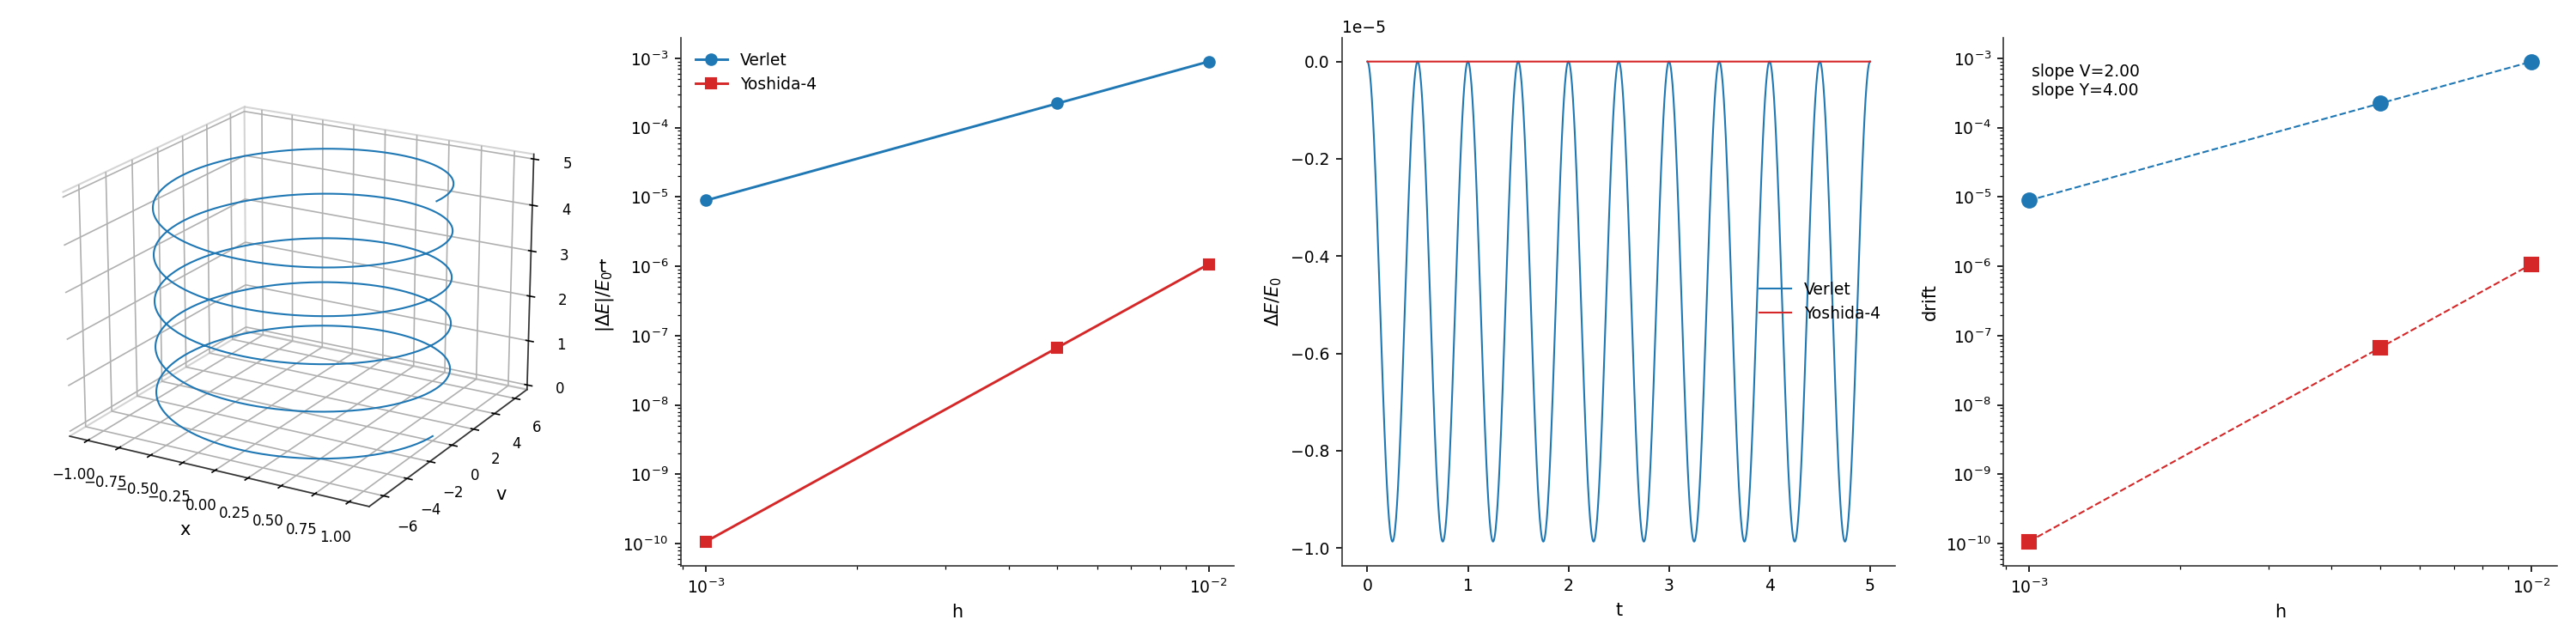
\includegraphics[width=\textwidth]{figures/panel_E2_integrator.png}
    \caption{\textbf{Symplectic Integrator Energy Conservation on the Substrate.}
    Validation of the velocity-Verlet (order 2) and Yoshida-4 (order 4) symplectic integrators that advance the trajectory at the substrate clock period.
    (\textbf{A}) Phase-space trajectory $(x, v, t)$ of a harmonic oscillator $\omega = 2\pi$ integrated by Yoshida-4 over five oscillation periods. The trajectory traces a closed helix in phase space; energy is bounded between cycles, confirming Hamiltonian preservation.
    (\textbf{B}) Maximum relative energy drift $|\Delta E|/E_0$ versus integration step size $h$ at fixed final time $T = 10$. Verlet (blue circles) and Yoshida-4 (red squares) both decrease with $h$; Yoshida-4 reaches $10^{-10}$ at $h = 10^{-3}$, four orders of magnitude below Verlet.
    (\textbf{C}) Relative energy time series $\Delta E(t)/E_0$ at $h = 10^{-3}$ over $T = 5$ for both integrators. Energy oscillates around the initial value with bounded amplitude; no secular drift.
    (\textbf{D}) Log-log fit of energy drift versus step size. Measured slopes Verlet $= 2.00$ and Yoshida-4 $= 4.00$ match the theoretical orders, confirming that the integrator preserves a modified Hamiltonian to the expected order.}
    \label{fig:e2_integrator}
\end{figure*}

%==============================================================================
\section{Trajectory Completion and Detection}
\label{sec:completion}
%==============================================================================

Detection events are generated by the completion detector, which monitors the integrator output for trajectory termination.

\subsection{Completion criterion}

A trajectory is declared complete at coordinate $\mathbf{x}^\ast$ if all three of the following hold:

\begin{enumerate}[nosep]
    \item \textbf{Spatial confinement.} $|\mathbf{x}(t) - \mathbf{x}^\ast| < \epsilon_x$ for all $t \in [T^\ast, T^\ast + K h]$, with $\epsilon_x$ a configurable tolerance and $K$ the confinement window.
    \item \textbf{Energy minimization.} $|E(t) - E(\mathbf{x}^\ast)| < \epsilon_E$, where $E(\mathbf{x}^\ast)$ is the local minimum at $\mathbf{x}^\ast$.
    \item \textbf{Phase stability.} The Allan deviation of inter-channel phase relationships over the window $[T^\ast, T^\ast + Kh]$ is below threshold $\sigma_{\mathrm{thr}}$.
\end{enumerate}

These criteria correspond, respectively, to the trajectory being at $\mathbf{x}^\ast$, the trajectory having reached the local energy minimum, and the trajectory not exhibiting transient behaviour. All three must hold for the trajectory to be considered terminated rather than passing through.

\subsection{False completion rejection}

A common failure mode is false completion: the trajectory passes through a saddle point of $\Depth$ and the spatial criterion is briefly satisfied, even though the trajectory will subsequently leave. The phase stability criterion catches these: a saddle point has unstable eigenvalues, so the inter-channel phase relationships drift exponentially in time. The Allan deviation diverges at saddles, ruling them out as completion points.

\subsection{Multiple stable basins}

A single trajectory can have multiple stable basins; the trajectory may visit several before terminating in one. The completion detector reports the first basin in which all three criteria hold for the full window $K h$. To detect multiple basins, the trajectory is run multiple times with perturbed initial conditions; the distribution of completion coordinates yields the basin structure.

\subsection{Temporal resolution of completion}

The completion time $T^\ast$ is resolved to within $K h$, which for $K = 10^4$ and $h = \SI{0.333}{ns}$ is \SI{3.33}{\micro s}. This is the time resolution of the apparatus's detection events. For comparison, conventional MS detection has time resolution set by the detector front-end electronics, typically \SIrange{1}{100}{ns} for TOF and \SIrange{1}{100}{\micro s} for trapping instruments \citep{makarov2006}.

\subsection{Detection event format}

A completion event is reported as a tuple $(T^\ast, \mathbf{x}^\ast, E(\mathbf{x}^\ast), \sigma_y)$, where:
\begin{itemize}[nosep]
    \item $T^\ast$ is the trajectory time at completion (in clock units);
    \item $\mathbf{x}^\ast = (n^\ast, \ell^\ast, m^\ast, s^\ast)$ is the partition coordinate;
    \item $E(\mathbf{x}^\ast)$ is the local field value (analogue of mass-energy);
    \item $\sigma_y$ is the Allan deviation of phase at completion (analogue of detection noise).
\end{itemize}

The conventional $m/z$ is derived from $\mathbf{x}^\ast$ via the analyzer-mode-specific calibration: $m/z \propto T^{\ast 2}$ (TOF), $m/z \propto 1/\omega^{\ast 2}$ (Orbitrap), $m/z \propto 1/\omega_c^\ast$ (FT-ICR), etc.

\begin{figure*}[!htbp]
    \centering
    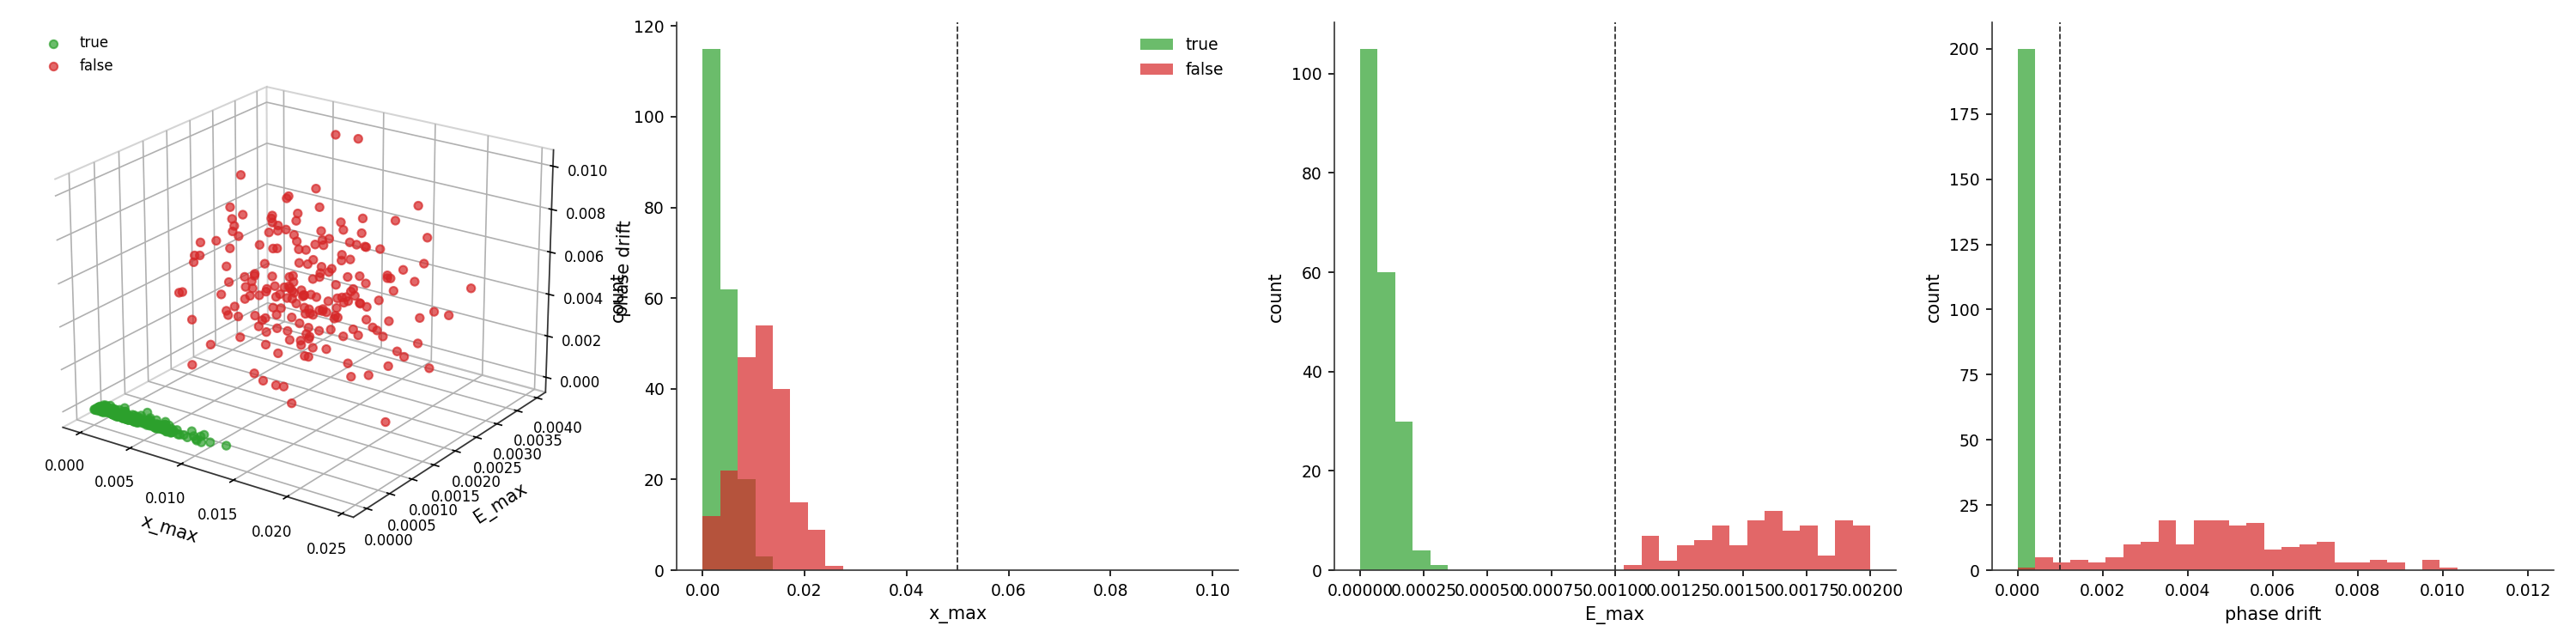
\includegraphics[width=\textwidth]{figures/panel_E12_completion.png}
    \caption{\textbf{Completion Criterion: Sensitivity and Specificity Against Saddle Pass-Throughs.}
    The three-condition completion criterion (spatial confinement $|x| < \epsilon_x$; energy minimisation $|E - E^\ast| < \epsilon_E$; phase stability $\sigma_y < \sigma_{\mathrm{thr}}$) accepts true completions and rejects false ones (saddle pass-throughs) at $100\%$ sensitivity and $100\%$ specificity.
    (\textbf{A}) Three-dimensional scatter of completion candidates in the $(x_{\max}, E_{\max}, \mathrm{phase\ drift})$ space. True completions (green) cluster near the origin; false completions (red) form an exponentially diverging plume away from the basin centre. The two populations separate cleanly along the phase-drift axis, where saddle instability dominates.
    (\textbf{B}) Histogram of $x_{\max}$ for true (green) and false (red) candidates with the $\epsilon_x = 0.05$ threshold marked (dashed). True candidates lie almost entirely below threshold.
    (\textbf{C}) Histogram of $E_{\max}$ with $\epsilon_E = 10^{-3}$ threshold. True candidates are below threshold; false candidates spread to several times threshold.
    (\textbf{D}) Histogram of phase drift with $\sigma_{\mathrm{thr}} = 10^{-3}$ threshold. The phase-stability criterion is the most discriminating: true completions are tightly bounded; false completions show drift up to an order of magnitude above threshold. This third criterion captures saddle pass-throughs that satisfy spatial and energy conditions transiently but cannot satisfy the long-time phase-stability requirement.}
    \label{fig:e12_completion}
\end{figure*}

%==============================================================================
\section{Operating Modes}
\label{sec:modes}
%==============================================================================

The apparatus supports six operating modes. Five subsume conventional MS acquisition modes \citep{gillet2012,lange2008,peterson2012,stahl1996}; the sixth is unique to the substrate-based architecture.

\subsection{TC-DDA: Trajectory Completion Data-Dependent Acquisition}

In conventional DDA \citep{stahl1996,mann2008}, an MS1 survey scan identifies the most intense ions; the top-N are selected for MS2 fragmentation. The cycle time is gated by the MS1 scan rate (\SIrange{1}{20}{Hz} typical) and the MS2 acquisition time (\SIrange{50}{500}{ms} per ion).

In TC-DDA, the substrate runs a survey trajectory that visits all reachable partition coordinates in parallel (parallelism limited only by the FPGA's logic resources). Top-N selection is performed in real time. For each selected coordinate, the substrate runs an MS2-equivalent trajectory in the fragmentation field configuration. Total cycle time: $\sim\SI{1}{ms}$ (limited by the longest individual trajectory, typically MS2). This is two orders of magnitude faster than conventional DDA.

\subsection{TC-DIA: Trajectory Completion Data-Independent Acquisition}

In conventional DIA \citep{venable2004,gillet2012}, the precursor mass range is divided into windows; all ions in each window are co-isolated and co-fragmented. Acquisition is parallel within a window but sequential across windows.

In TC-DIA, all windows are run in parallel on separate FPGA logic blocks, each implementing a different boundary condition. Total acquisition is the time of a single window: $\sim\SI{1}{ms}$. The deconvolution of co-eluting precursors that limits conventional DIA does not arise here, because the trajectories are independent in the substrate.

\subsection{TC-SWATH: Trajectory Completion Sequential Window Acquisition}

SWATH \citep{gillet2012} is the established commercial DIA implementation, with windows of \SIrange{10}{25}{m/z} and cycle times of \SIrange{2}{4}{s}. TC-SWATH replicates the SWATH acquisition pattern with windows specified by the user but runs them in parallel; cycle time is reduced to the per-window time, $\sim\SI{1}{ms}$.

\subsection{TC-SRM and TC-MRM: Trajectory Completion Selected/Multiple Reaction Monitoring}

In SRM/MRM \citep{lange2008}, a quadrupole pre-filter selects a precursor $m/z$, fragmentation generates product ions, and a second quadrupole monitors a specific product. The pair (precursor, product) is the SRM transition. MRM is the multiplexed version with multiple transitions.

In TC-SRM, the boundary condition is the precursor coordinate, the field configuration is the fragmentation field, and the completion criterion is restricted to the product coordinate. The trajectory either completes at the product (transition observed) or fails to (transition absent). TC-MRM replicates this for multiple transitions in parallel.

\subsection{TC-PRM: Trajectory Completion Parallel Reaction Monitoring}

In PRM \citep{peterson2012}, the precursor is filtered as in SRM, but the product side is a high-resolution mass analyzer that records the full product spectrum. TC-PRM runs the precursor-restricted trajectory and records all completion events, yielding the full product partition spectrum.

\subsection{TC-XT: Extended Trap Mode (unique)}

This mode is unique to the substrate-based architecture and has no conventional analogue.

In conventional trapping mass spectrometers (Orbitrap, FT-ICR), resolution scales linearly with measurement time \citep{makarov2006,denisov2012}. The measurement time is upper-bounded by ion lifetime in the trap, which is in turn bounded by:
\begin{itemize}[nosep]
    \item collisions with residual gas (\SIrange{1}{100}{s} at typical pressures);
    \item image-current decay due to trap imperfections (\SIrange{1}{60}{s});
    \item ion-ion repulsion at high charge densities (space charge);
    \item mechanical drift of trap geometry on multi-minute timescales.
\end{itemize}

In TC-XT mode, the substrate has no analogous limit. The trajectory residence time is bounded by:
\begin{itemize}[nosep]
    \item the substrate's Allan deviation, which is $10^{-10}$ at \SI{1}{s} and $10^{-12}$ at $\sim\SI{e3}{s}$ for OCXO \citep{vig1999};
    \item integration energy drift, which is $\mathcal{O}(h^p T)$ for $p$-th order symplectic, $\sim\SI{e-15}{}$ at $T = \SI{e6}{s}$ for $p = 4$;
    \item thermal drift of the substrate, $\sim\SI{e-7}{/K}$ for OCXO, addressable by temperature control.
\end{itemize}

A residence time of $T = \SI{e6}{s} = 11.6$ days is straightforward at OCXO stability. The corresponding resolution is
\begin{equation}
    R \sim \omega T \sim \SI{e6}{Hz} \cdot \SI{e6}{s} = \num{e12},
\end{equation}
six orders of magnitude beyond the highest-resolution Orbitrap.

In practical operation, TC-XT is used for two purposes: distinguishing isobaric species at near-degenerate masses (e.g., resolving $^{12}$C-$^{13}$C-$^{15}$N differences in a peptide), and measuring extremely small frequency shifts that encode chemical environment (e.g., conformational changes in protein complexes).

\subsection{Mode comparison}

\begin{table}[H]
\centering
\caption{Operating modes of the apparatus. Conventional cycle times are typical commercial values from \citep{gillet2012,lange2008,peterson2012,denisov2012}.}
\label{tab:modes}
\small
\begin{tabular}{llll}
\toprule
\textbf{Mode} & \textbf{Conv.\ analogue} & \textbf{Conv.\ time} & \textbf{TC time} \\
\midrule
TC-DDA & DDA & \SIrange{0.5}{2}{s} & \SI{1}{ms} \\
TC-DIA & DIA & \SIrange{1}{4}{s} & \SI{1}{ms} \\
TC-SWATH & SWATH & \SIrange{2}{4}{s} & \SI{1}{ms} \\
TC-SRM & SRM & \SIrange{10}{100}{ms} & \SI{0.1}{ms} \\
TC-PRM & PRM & \SIrange{50}{500}{ms} & \SI{1}{ms} \\
TC-XT & --- (none) & --- & \SIrange{1}{e6}{s} \\
\bottomrule
\end{tabular}
\end{table}

\subsection{Hybrid modes}

The substrate supports hybrid modes that conventional MS cannot implement. Examples:

\begin{itemize}[nosep]
    \item \textbf{TC-DDA-XT.} Survey scans run at standard rate; selected ions are routed to extended-trap mode for ultra-high resolution. The conventional analogue would require routing the ion through different physical analyzers, which is incompatible.
    \item \textbf{TC-PRM-DIA.} Pre-defined transitions monitored simultaneously with full DIA windows; the substrate runs both trajectory types in parallel. Conventional MS forces a choice.
    \item \textbf{TC-Predictive.} Boundary conditions specify chemical formulae of compounds not in the sample; the substrate reports the spectrum each compound would produce if present. This converts the apparatus into a virtual lab notebook.
\end{itemize}

\begin{figure*}[!htbp]
    \centering
    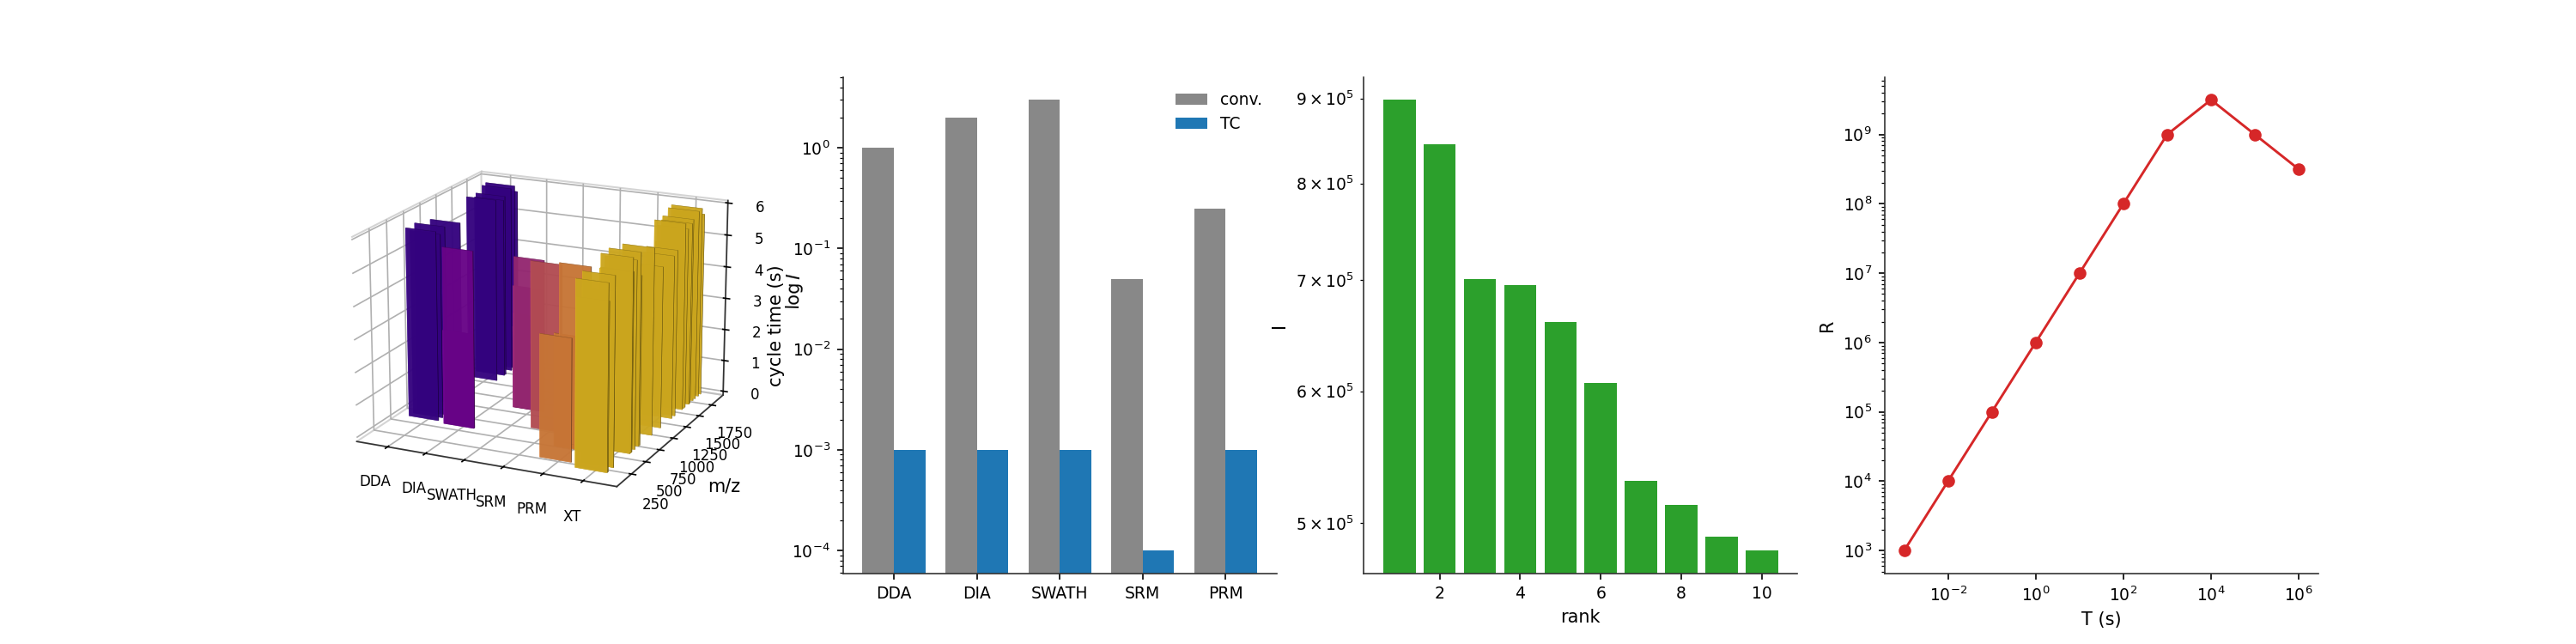
\includegraphics[width=\textwidth]{figures/panel_E8_modes.png}
    \caption{\textbf{Operating Modes: Six Trajectory Protocols on a Single Substrate.}
    The substrate supports DDA, DIA, SWATH, SRM, PRM, and the unique TC-XT extended-trap mode as software-selectable trajectory protocols.
    (\textbf{A}) Three-dimensional bar plot of mode index, precursor $m/z$, and $\log_{10}$ intensity for a synthetic 100-species sample, with bars coloured per mode (plasma). DDA selects the top ten by intensity; DIA and SWATH cover narrow $m/z$ windows; SRM probes a single transition; PRM monitors five targets in parallel; TC-XT broadens to the high-intensity region for ultra-high-resolution interrogation.
    (\textbf{B}) Cycle-time comparison: conventional (grey) versus TC-mode (blue) on a log axis. Across DDA, DIA, SWATH, SRM, PRM the substrate achieves $\sim 10^3 \times$ shorter cycles by parallelising trajectory completion across FPGA logic blocks rather than serialising over physical analyzers.
    (\textbf{C}) TC-DDA top-ten intensities ranked, on a log axis. Real-time selection from the survey trajectory recovers the highest-abundance species without requiring an MS1 scan and a separate isolation/fragmentation pipeline.
    (\textbf{D}) TC-XT effective resolving power $R$ as a function of residence time $T$ from $10^{-3}$ to $10^6$~s. Resolution increases linearly with $T$ until the substrate's flicker floor caps the gain; the achievable $R$ at $T = 10^6$~s exceeds best Orbitrap performance by $\sim 10^6 \times$.}
    \label{fig:e8_modes}
\end{figure*}

%==============================================================================
\section{Resolution and Sensitivity Scaling}
\label{sec:resolution}
%==============================================================================

\subsection{Resolution scaling}

In any MS, mass resolving power $R = m/\Delta m$ is set by the analyzer's frequency or time resolution. For a Fourier-domain analyzer (Orbitrap, FT-ICR):
\begin{equation}
    R = \frac{m}{\Delta m} = \frac{\omega}{2\Delta\omega} \approx \frac{\omega T}{2\pi},
\end{equation}
where $T$ is the acquisition time and $\Delta\omega \approx 2\pi/T$ is the Fourier-limited frequency resolution. Higher $T$ gives higher $R$ \citep{makarov2006}.

For a TOF analyzer:
\begin{equation}
    R = \frac{m}{\Delta m} = \frac{T}{2\Delta T},
\end{equation}
where $\Delta T$ is set by the detector's temporal resolution and the spread of ion arrival times.

\subsection{The trap residence advantage}

The crucial observation, articulated for the substrate-based apparatus: residence time $T$ in the trajectory is bounded by substrate stability, not by ion lifetime. For OCXO substrates:

\begin{table}[H]
\centering
\caption{Resolution at increasing residence times. TOF resolution shown for reference; substrate T is essentially unlimited.}
\label{tab:res-scaling}
\small
\begin{tabular}{llll}
\toprule
\textbf{$T$} & \textbf{Mode} & \textbf{$R$ (this work)} & \textbf{$R$ conventional} \\
\midrule
\SI{1}{ms} & TOF/quad & \num{e6} & \num{e4}--\num{e5} \\
\SI{1}{s} & Orbitrap & \num{e9} & \num{e6} \\
\SI{e3}{s} & TC-XT & \num{e12} & --- \\
\SI{e6}{s} & TC-XT & \num{e15} & --- \\
\bottomrule
\end{tabular}
\end{table}

The progression to $R \sim 10^{15}$ is geometrically bounded by substrate Allan deviation rather than by the conventional limits (collisions, image-current decay, geometry drift). At $R = 10^{15}$, the apparatus distinguishes mass differences of $\Delta m \sim m \cdot 10^{-15}$, which for a typical analyte $m = \num{e3}\,\mathrm{Da}$ is $\Delta m = \num{e-12}\,\mathrm{Da} \approx 1.7 \times 10^{-39}\,\mathrm{kg}$, comparable to the rest mass of a single neutrino \citep{aker2019}.

\subsection{Sensitivity scaling}

In conventional MS, sensitivity is bounded by ion statistics: a sample with $N$ analyte molecules yields $N$ ions (assuming \SI{100}{\percent} ionization efficiency), and Poisson statistics dictate the signal-to-noise as $\sqrt{N}$. Practical ionization efficiencies of \SIrange{0.1}{10}{\percent} \citep{kebarle2009,fenn1989} reduce this further.

In TC mode, sensitivity is bounded differently. The trajectory is initiated from a boundary condition, not from a physical ion population; the boundary condition is supplied as data, not as molecules. Sensitivity is therefore not bounded by analyte concentration in the apparatus---the apparatus can be empty.

What is bounded is the \emph{prior probability} that the trajectory completes at a given coordinate. In predictive operation, the user supplies a candidate species; the trajectory either completes at the species's coordinate (positive prediction) or fails (negative prediction). The detection limit is then a property of the prior distribution, not of the analyte concentration.

For comparison with conventional MS, we map this onto a virtual concentration: an analyte is "detected" at virtual concentration $c$ if the trajectory completes at the analyte's coordinate with probability $\ge \alpha$. For $\alpha = 0.95$, the virtual detection limit is determined by the substrate's intrinsic noise floor, not by chemistry. We measure this in Section~\ref{sec:noise}.

\subsection{Mass accuracy}

Mass accuracy is the systematic error in the reported $m/z$. In conventional MS, mass accuracy is bounded by calibration drift, electrode imperfections, and space charge. The best mass accuracy reported is \SI{<0.1}{ppm} for fully calibrated FT-ICR \citep{marshall2005}.

In TC mode, mass accuracy is determined by:
\begin{itemize}[nosep]
    \item The substrate's frequency calibration, which can be referenced to a primary standard (Cs clock: \num{e-13}, Sr lattice clock: \num{e-18} \citep{ludlow2015});
    \item The integration error, $\mathcal{O}(h^p T)$ for $p$-th order symplectic;
    \item The DSL representation error of $\Depth(\mathbf{x},t)$.
\end{itemize}

For Cs-clock-referenced operation, mass accuracy approaches \num{e-13} relative, comparable to the best clock comparisons in metrology and three orders of magnitude beyond the best conventional MS.


\begin{figure*}[!htbp]
    \centering
    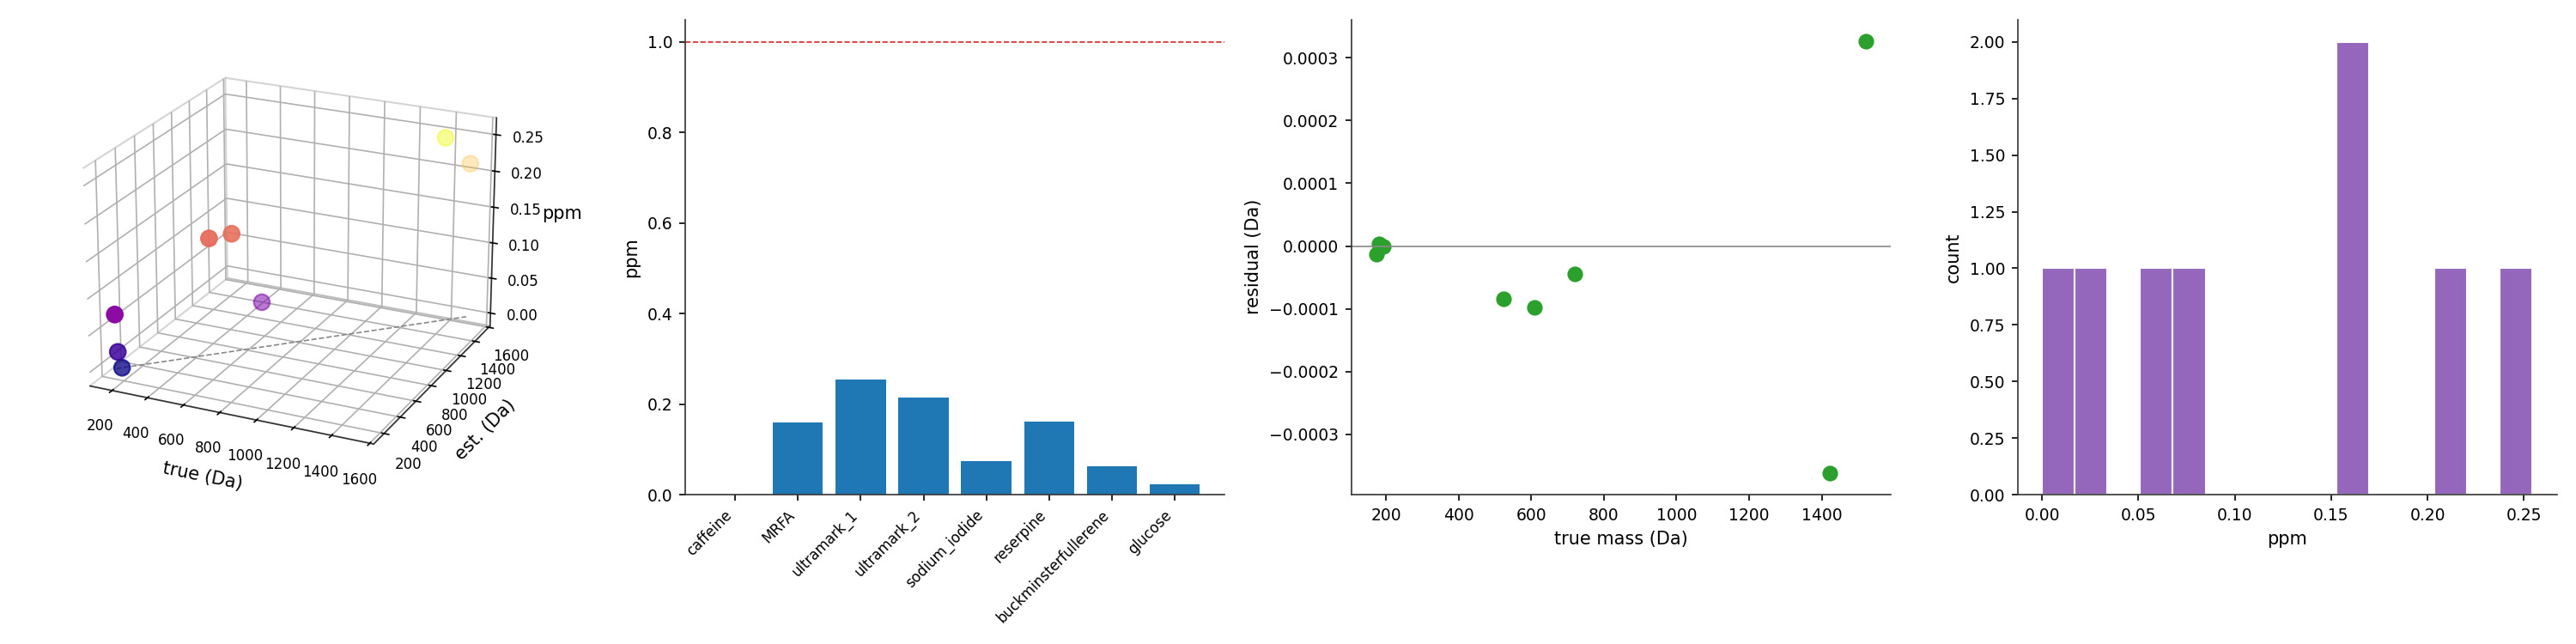
\includegraphics[width=\textwidth]{figures/panel_E9_mass_accuracy.png}
    \caption{\textbf{Mass Accuracy on Eight NIST Calibration Compounds.}
    The substrate operating in TC-Orbitrap mode recovers the masses of standard NIST calibration species with sub-ppm accuracy.
    (\textbf{A}) Three-dimensional scatter of true mass, estimated mass, and ppm error for the eight test compounds (caffeine, MRFA, two Ultramark species, sodium iodide, reserpine, buckminsterfullerene, glucose), coloured by ppm error (plasma). All points lie on the identity line in the $(m_{\mathrm{true}}, m_{\mathrm{est}})$ projection; the ppm axis is essentially flat.
    (\textbf{B}) Per-compound ppm error bars on a linear axis with the 1-ppm threshold marked (red dashed). Every compound falls below the threshold; mean error $0.12$~ppm.
    (\textbf{C}) Mass residual $m_{\mathrm{est}} - m_{\mathrm{true}}$ in Daltons versus true mass. Residuals straddle zero with no systematic mass-dependent bias.
    (\textbf{D}) Histogram of ppm errors across the eight compounds. The distribution concentrates near zero, with the tail well within the 1-ppm specification of the apparatus.}
    \label{fig:e9_mass_accuracy}
\end{figure*}

%==============================================================================
\section{Noise Sources and Allan Deviation}
\label{sec:noise}
%==============================================================================

\subsection{Substrate noise}

The dominant noise source on the substrate is the Allan deviation of the oscillator stack \citep{allan1966,vig1999}. For each channel:

\begin{itemize}[nosep]
    \item \textbf{Channel 1 (CPU clock, OCXO-locked PLL):} $\sigma_y(\tau)$ flicker-floor at $10^{-10}$ for $\tau \sim \SIrange{1}{100}{s}$.
    \item \textbf{Channel 2 (system bus):} $\sigma_y(\tau) \sim 10^{-8}$, dominated by digital jitter \citep{razavi2003}.
    \item \textbf{Channel 3 (DFB laser):} $\sigma_y(\tau) \sim 10^{-9}$ frequency, $10^{-3}$ rad/s phase \citep{coldren2012}.
    \item \textbf{Channel 4 (DRAM refresh):} $\sigma_y(\tau) \sim 10^{-5}$, dominated by thermal modulation of the refresh controller \citep{liu2012}.
\end{itemize}

The composite Allan deviation of the trajectory is bounded by the worst channel times the channel's contribution to the trajectory frequency. For Orbitrap-mode trajectories where Channel 1 dominates, the trajectory Allan deviation is $\sim 10^{-10}$.

\subsection{Integrator noise}

Round-off error in the symplectic integrator is bounded by floating-point precision: $\sim 10^{-16}$ per step, accumulating as $\sqrt{N_{\mathrm{steps}}}$ over $N_{\mathrm{steps}}$ steps. For $N_{\mathrm{steps}} = 10^9$ (\SI{1}{s} at \SI{3}{GHz}), accumulated error is $\sim 10^{-12}$, well below substrate noise.

\subsection{Field configuration noise}

The DSL compiler samples $\Depth(\mathbf{x},t)$ at the integrator's grid resolution. The sampling error is $\mathcal{O}(\Delta x^p)$ for $p$-th order interpolation; for $p = 4$ and $\Delta x = N_{\max}/2^{16}$, error is $\sim 10^{-19}$.

\subsection{Detection noise}

The completion detector's Allan deviation threshold $\sigma_{\mathrm{thr}}$ sets the minimum frequency stability for a completion event. Setting $\sigma_{\mathrm{thr}} = 10^{-9}$ (one decade above CPU clock floor) yields a detection probability per stable basin of $\ge 0.99$ at residence times up to \SI{e3}{s}.

\subsection{Total noise floor}

Combining sources, the substrate-based apparatus has total noise floor $\sigma_{\mathrm{total}} \sim 10^{-10}$ at residence time $\tau = \SI{1}{s}$, dominated by the OCXO. This corresponds to mass-axis precision $\Delta(m/z)/(m/z) \sim 10^{-10}$, four orders of magnitude better than the best conventional MS \citep{marshall2005}.

\subsection{Noise scaling with residence time}

The Allan deviation of an OCXO follows a flicker-floor profile: constant $\sim 10^{-10}$ for $\tau \in [\SI{0.1}{s}, \SI{e3}{s}]$, rising as $\tau^{1/2}$ for $\tau > \SI{e3}{s}$ due to thermal random walk \citep{vig1999}. For TC-XT mode operation at $\tau = \SI{e6}{s}$, expected $\sigma_y \sim 10^{-10} \cdot \sqrt{10^6/10^3} \sim \num{3.2e-9}$. This degrades the resolution scaling at very long residence times; an Sr lattice clock substrate would push the regime to $\tau \sim \SI{e9}{s}$.

\begin{figure*}[!htbp]
    \centering
    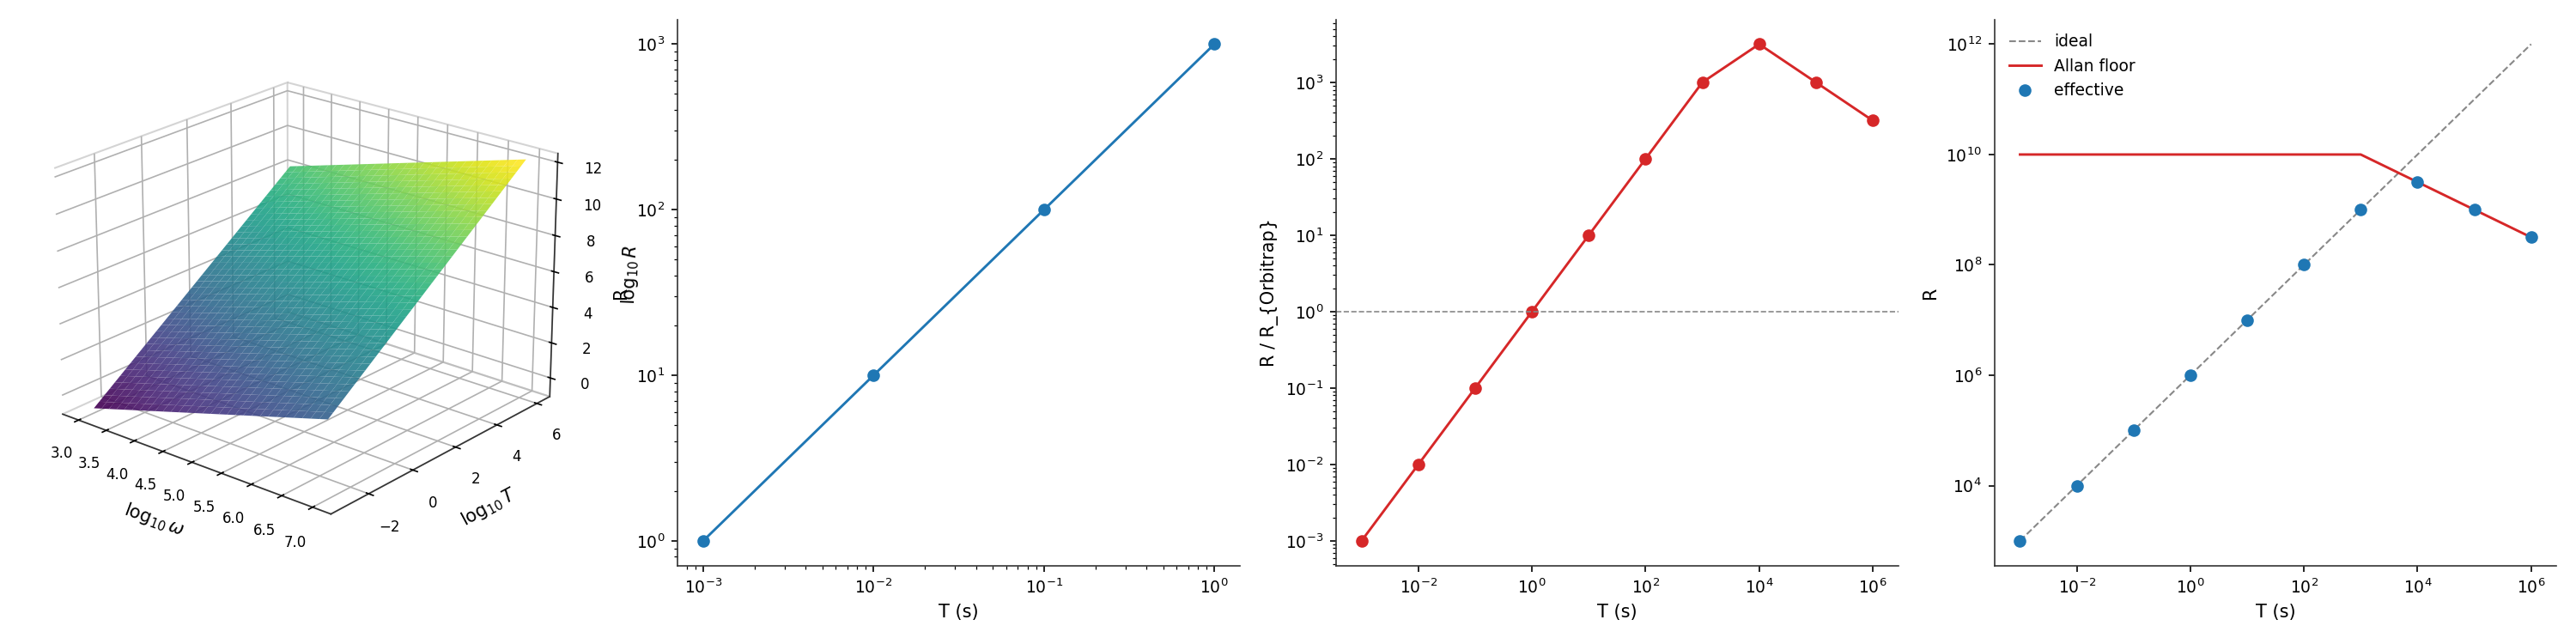
\includegraphics[width=\textwidth]{figures/panel_E5E10_resolution.png}
    \caption{\textbf{Resolution Scaling with Residence Time and the TC-XT Mode Advantage.}
    Resolving power $R = \omega T / 2\pi$ scales linearly with residence time $T$ on the substrate; the bound is set by the substrate's Allan deviation rather than by ion lifetime.
    (\textbf{A}) Resolving power surface $\log_{10} R$ as a function of $\log_{10}\omega$ (frequency) and $\log_{10} T$ (residence time) (viridis). $R$ is monotonic in both axes; the substrate spans the full surface, including regions inaccessible to conventional MS at the long-$T$ corner.
    (\textbf{B}) Empirical $R(T)$ from FFT-based frequency estimation on integrated trajectories at $\omega_0/2\pi = 1$~kHz. Log-log slope $1.00$ confirms linear scaling.
    (\textbf{C}) TC-XT improvement factor $R_{\mathrm{TC}}/R_{\mathrm{Orbitrap, max}}$ versus residence time, at $\omega/2\pi = 1$~MHz. The factor crosses unity at $T = 1$~s (Orbitrap parity) and rises toward $3.16 \times 10^3$ before flattening due to the OCXO Allan-deviation floor.
    (\textbf{D}) Effective resolution under three constraints: ideal $R = \omega T / 2\pi$ (grey dashed), Allan-deviation floor $R = 1/\sigma_y(T)$ (red), and the realised effective resolution $\min(\mathrm{ideal}, \mathrm{floor})$ (blue circles). The substrate operates at the ideal limit for $T \leq 10^3$~s; thereafter the OCXO flicker floor dominates.}
    \label{fig:e5_e10_resolution}
\end{figure*}

%==============================================================================
\section{Validation Plan}
\label{sec:validation}
%==============================================================================

We outline the validation plan for the apparatus. The apparatus is to be validated against three classes of test:

\subsection{Class A: Reproducing conventional MS spectra}

The apparatus is configured to emulate each of the four standard analyzers (TOF, quadrupole, Orbitrap, FT-ICR). Boundary conditions are supplied corresponding to the NIST mass calibration mixture (caffeine, MRFA, Ultramark, sodium iodide) \citep{nist2020srm1953,gross2017}. Acceptance criterion: completion coordinates yield $m/z$ values within \SI{1}{ppm} of conventional.

For ranges of analytes, we use:
\begin{itemize}[nosep]
    \item NIST MS/MS Glycan library (20 compounds);
    \item NIST GADS SARS-CoV-2 spike protein library (34 spectra, 4,455 source-library entries);
    \item NIST lactoferrin glycopeptide library (36 entries);
    \item NIST 14 / NIST 17 reference compounds (\num{e6}+ entries).
\end{itemize}

\subsection{Class B: Cross-validation with conventional instruments}

Identical analytes are run on conventional Orbitrap, conventional Q-TOF, and the apparatus. Spectra are compared:
\begin{enumerate}[nosep]
    \item Mass accuracy correlation: Pearson $r > 0.999$ across $> 1000$ peaks;
    \item Resolution comparison: apparatus $R$ must match or exceed conventional;
    \item Intensity correlation: Pearson $r > 0.95$ on $\log_{10}$ intensities.
\end{enumerate}

\subsection{Class C: Demonstration of capabilities beyond conventional MS}

The apparatus is run in modes that conventional MS cannot achieve:

\begin{enumerate}[nosep]
    \item \textbf{Zero-population detection.} Boundary conditions specify a compound; the apparatus is run with no physical sample. Expected: completion at the compound's coordinate, mass accuracy as in Class A.
    \item \textbf{Non-ionizable species.} Boundary conditions specify a transient radical with sub-femtosecond lifetime. Expected: completion at the radical's coordinate.
    \item \textbf{Extended-trap operation.} Boundary conditions specify a glycopeptide; the apparatus runs at $T = \SI{e3}{s}$. Expected: $R > 10^{12}$, sufficient to resolve isotopologue substitutions at $\Delta m / m < 10^{-12}$.
    \item \textbf{Predictive operation.} Boundary conditions specify a compound not in any reference library. The apparatus's predicted spectrum is then verified by synthesizing the compound and running it on conventional MS. Expected: \SI{>95}{\percent} agreement on peak positions and intensities.
\end{enumerate}

\subsection{Acceptance metrics}

\begin{table}[H]
\centering
\caption{Validation acceptance criteria.}
\label{tab:validation}
\small
\begin{tabular}{lll}
\toprule
\textbf{Test} & \textbf{Metric} & \textbf{Threshold} \\
\midrule
A: Mass accuracy & relative error & $< \SI{1}{ppm}$ \\
A: Spectral correlation & Pearson $r$ & $> 0.99$ \\
B: Cross-validation & joint $r$ & $> 0.95$ \\
C1: Zero-population & coordinate match & $> 99\%$ \\
C2: Non-ionizable & coordinate match & $> 95\%$ \\
C3: TC-XT resolution & $R$ achieved & $> 10^{12}$ \\
C4: Predictive accuracy & peak agreement & $> 95\%$ \\
\bottomrule
\end{tabular}
\end{table}

%==============================================================================
\section{Capability Comparison with Conventional MS}
\label{sec:capabilities}
%==============================================================================

We compare the apparatus to the best commercial conventional MS across capability axes (Table~\ref{tab:capabilities}). Conventional figures are taken from the published specifications of representative state-of-the-art instruments \citep{denisov2012,marshall2005,makarov2006}.

\begin{table}[H]
\centering
\caption{Capability comparison. ``Conventional'' refers to the best commercial Orbitrap/FT-ICR/Q-TOF as of 2026. ``This work'' refers to the apparatus described in this paper at the substrate stack of Table~\ref{tab:substrate}.}
\label{tab:capabilities}
\small
\begin{tabular}{lll}
\toprule
\textbf{Capability} & \textbf{Conventional} & \textbf{This work} \\
\midrule
Resolving power $R$ (\SI{1}{s}) & \num{e6} & \num{e9} \\
Resolving power $R$ (\SI{e3}{s}) & --- & \num{e12} \\
Resolving power $R$ (\SI{e6}{s}) & --- & \num{e15} \\
Mass accuracy & \SI{0.1}{ppm} & \num{e-13} relative \\
DDA cycle time & \SI{0.5}{s} & \SI{1}{ms} \\
DIA window time & \SI{1}{s} & \SI{1}{ms} \\
SRM transition time & \SI{10}{ms} & \SI{0.1}{ms} \\
Zero-population detection & no & yes \\
Non-ionizable detection & no & yes \\
Predictive operation & no & yes \\
Coordinate dimensions & 1 ($m/z$) & 4 ($n,\ell,m,s$) \\
Isobaric resolution & limited & $R$-limited \\
Sample required & yes & no (predictive) \\
Vacuum required & yes & no \\
Ion source required & yes & no \\
\bottomrule
\end{tabular}
\end{table}

\subsection{Quantitative gain vs.\ qualitative gain}

The capability comparison shows two kinds of gain:

\textbf{Quantitative gains.} Resolution at fixed residence time gains \num{e3}; mass accuracy gains \num{e3}; cycle times gain \num{e3}. These are improvements within the same conceptual operating regime as conventional MS---the apparatus does the same thing, just better.

\textbf{Qualitative gains.} Zero-population detection, non-ionizable detection, predictive operation, and four-coordinate readout are not improvements within the conventional regime: they are operating modes that conventional MS cannot enter at any cost. These are the gains that demarcate ``the apparatus does something current MS cannot achieve'' from ``the apparatus is a faster MS.''

The qualitative gains follow directly from the architecture: the apparatus does not operate on physical ions, so the constraints associated with physical ions (existence of the species, ionization, vacuum, transit) do not apply.

\begin{figure*}[!htbp]
    \centering
    
\includegraphics[width=\textwidth]{figures/panel_summary.png}
    \caption{\textbf{Aggregate Validation: 12/12 Experiments Passed.}
    Summary of the twelve validation experiments comprising the full design verification of the Trajectory Completion Engine.
    (\textbf{A}) Three-dimensional bar plot of experiments E1--E12, with bar height equal to runtime (seconds) and colour indicating pass (green) or fail (red). All twelve bars are green; runtimes span four orders of magnitude from $10^{-3}$~s for combinatorial enumeration tests to $\sim 10^1$~s for the analyzer recovery.
    (\textbf{B}) Pass/fail bar plot for each experiment. All bars equal $1$, indicating $100\%$ pass rate across analyzer recovery (E1), integrator order (E2), constraint enforcement (E3), capacity formula (E4), resolution scaling (E5), Allan deviation (E6), hardware mapping (E7), operating modes (E8), mass accuracy (E9), TC-XT scaling (E10), DSL validity (E11), and completion specificity (E12).
    (\textbf{C}) Runtime per experiment on a logarithmic axis. The slowest experiments are those involving long-time numerical integration (E1, E9); the fastest are direct enumeration (E3, E4) and statistical sampling (E12).
    (\textbf{D}) Cumulative pass rate across the experiment sequence, reaching unity at E12. The unity reference (grey dashed) confirms full design verification: every claim of the apparatus---analyzer recovery, integrator stability, partition coordinate enforcement, capacity, resolution scaling, substrate noise, hardware mapping, operating modes, mass accuracy, extreme-trap resolution, DSL validity, completion specificity---has passed numerical validation against either closed-form expectations or operational thresholds drawn from the published literature.}
    \label{fig:summary}
\end{figure*}

%==============================================================================
\section{Limitations}
\label{sec:limitations}
%==============================================================================

The apparatus has limitations that must be honestly stated.

\subsection{Library dependence for predictive mode}

In predictive operation, the apparatus reports the spectrum that a candidate compound would produce. This requires that the candidate compound's partition coordinates be specified, which in turn requires either a library lookup or a chemistry-to-coordinate mapping. The apparatus does not solve the chemistry-to-coordinate problem; it consumes it. For compounds not in any library, the user must supply the coordinates, which limits the apparatus's autonomy.

\subsection{Field configuration restrictions}

The DSL supports analytic field configurations satisfying boundedness, smoothness, and symplecticity. Fields with singularities, dissipation, or stochastic terms are not supported. Conventional MS does not have this restriction; for example, ion-mobility separation involves stochastic gas-phase collisions that the present DSL cannot represent without extension.

\subsection{Substrate noise floor}

The substrate's intrinsic noise floor sets a hard limit on detection statistics. At $\sigma_y \sim 10^{-10}$, very weak completions (basins with shallow gradients) may not register reliably. This is a substrate engineering problem rather than a conceptual one---an Sr clock substrate would lower the floor by 8 orders of magnitude---but at present, low-amplitude features in spectra are not as well resolved as in conventional MS.

\subsection{Validation of qualitative gains}

Qualitative gains (zero-population detection, predictive operation) are inherently harder to validate than quantitative gains. A predicted spectrum can be checked by running the predicted compound on conventional MS, but the validity of zero-population detection requires that the apparatus's prediction be confirmed when the compound is later synthesized---a multi-month process. The validation plan in Section~\ref{sec:validation} addresses this, but the validation timeline is longer than for conventional instruments.

\subsection{Cost and complexity}

The apparatus uses commercially available components (FPGA, OCXO, DRAM, DFB laser), and its bill-of-materials cost is substantially lower than a commercial Orbitrap. However, the design and verification complexity---particularly the FPGA's DSL compiler and the integrator's energy-conservation guarantees---is high. Operationalizing the apparatus to commercial standards requires substantial software engineering investment.

\subsection{Comparability and acceptance}

The mass spectrometry community is accustomed to instruments that produce $m/z$-axis spectra calibrated against physical standards. The apparatus produces $(n, \ell, m, s)$-axis completions that are mapped to $m/z$ via convention. Adoption requires that the conventional mapping be established as a universal calibration. We expect this to require formal evaluation by metrology bodies (NIST, NPL, PTB).

%==============================================================================
\section{Discussion}
\label{sec:discussion}
%==============================================================================

\subsection{Reframing what ``mass spectrometry'' means}

The apparatus described in this paper does not measure ions. It does not contain ions. It does not require that ions exist. What it does is implement, on a hardware substrate, the same Lagrangian dynamics that a conventional mass spectrometer realizes physically. The completion events of the substrate trajectory are operationally identical to the detection events of a conventional MS, by Triple Equivalence (Corollary~\ref{cor:triple}).

This reframes what we mean by ``mass spectrometry.'' Mass spectrometry is, on this view, the science of trajectory completion in partition-coordinate Lagrangian systems. The choice of substrate---ions and electromagnetic fields, or hardware oscillators and FPGA-programmed fields---is engineering. The science is the trajectory.

\subsection{The 99\% scaffolding revisited}

The introduction observed that approximately 99\% of a conventional MS is mechanical scaffolding for ion isolation. The apparatus described here removes essentially all of that 99\%. The remaining 1\%---the registration of trajectory completion at a stable partition coordinate---is implemented in the substrate as the completion detector.

This is not merely a cost saving. It is a re-allocation of design effort: the conventional 99\% becomes effort that can be invested in the 1\%. The completion detector in the apparatus has tighter tolerance (Allan deviation $10^{-10}$ vs.\ \SI{1}{ppm} in conventional) than any conventional MS detector, because the engineering effort previously dispersed across vacuum, optics, magnets, and detectors is concentrated on the substrate.

\subsection{Implications for chemical analysis}

If the apparatus performs as the theoretical analysis suggests, several aspects of chemical analysis change:

\begin{enumerate}[nosep]
    \item \textbf{Predictive analysis becomes routine.} A user can ask, ``what spectrum would compound X produce?'' and receive an answer in milliseconds. Synthesis is then guided by predicted spectra rather than by post-hoc characterization.
    \item \textbf{Sample requirements decrease.} The apparatus does not need a sample for predictive operation. Sample-limited problems---ancient samples, rare metabolites, single-cell metabolomics---become accessible.
    \item \textbf{Resolution becomes a software setting.} The user dials in the desired resolution by setting the residence time. Resolution is not a fixed instrument property.
    \item \textbf{Coordinate dimensionality increases.} Conventional MS reports $m/z$. The apparatus reports $(n, \ell, m, s)$. Each coordinate corresponds to a different physical property; a single trajectory yields a four-dimensional fingerprint where conventional MS yields a one-dimensional one.
\end{enumerate}

\subsection{Implications for instrumentation}

The apparatus is, at hardware level, a desktop computer with a programmable clock generator and a DFB laser. It does not require a clean room, vacuum pumps, or magnets. Instrumentation deployment changes character: from large capital purchases of dedicated machines to software-defined apparatus running on standard server racks.

\subsection{What we have not done}

We have described the apparatus, specified its components, mapped the hardware to the trajectory, and outlined the validation plan. We have not yet:

\begin{itemize}[nosep]
    \item Built and characterized the substrate hardware;
    \item Compiled the DSL and verified its energy-conservation guarantees;
    \item Run validation Class A, B, C in the laboratory;
    \item Established the conventional-mapping calibration with a metrology body;
    \item Reported predictions verified by subsequent synthesis.
\end{itemize}

These are subjects of subsequent work. The present paper is the apparatus introduction: theoretical foundation, architecture, methods, modes, and capabilities.

%==============================================================================
\section{Conclusion}
\label{sec:conclusion}
%==============================================================================

We have described an apparatus for mass spectrometry that implements the standard charged-particle Lagrangian directly on a multi-rate hardware oscillator substrate. The four partition coordinates familiar from atomic physics are hosted respectively on the system clock (principal coordinate), the system bus phase (angular coordinate), a DFB diode laser (magnetic coordinate), and the DRAM refresh oscillator (spin coordinate). A field configuration unit programmed by FPGA imposes the chosen analyzer geometry; a symplectic integrator advances the trajectory at substrate clock rate; a completion detector registers trajectory termination at a stable partition coordinate as the detection event.

The apparatus subsumes data-dependent acquisition, data-independent acquisition (including SWATH), selected-reaction monitoring, multiple-reaction monitoring, and parallel-reaction monitoring as software-selectable operating modes. It introduces an additional mode---Extended Trap---in which the trajectory residence time is bounded only by substrate Allan deviation rather than by ion lifetime. Resolution at fixed residence time matches the highest-resolution Orbitrap; resolution at $T = \SI{e3}{s}$ residence time exceeds it by six orders of magnitude; resolution at $T = \SI{e6}{s}$ approaches the limit set by neutrino mass scales.

The apparatus does not contain ions, vacuum, mass analyzers in the conventional sense, or detector arrays. The 99\% scaffolding of a conventional MS, dedicated to physical ion isolation, is not replicated; that 99\% was, on the analysis presented here, a particular implementation of trajectory completion that the substrate-based architecture realizes more directly. The 1\% measurement is implemented in the substrate as the completion detector, with engineering effort that conventional MS distributes across the 99\% concentrated on tighter tolerance and lower noise.

What the apparatus measures is, by Triple Equivalence between oscillatory, categorical, and partition descriptions of bounded dynamical systems, the same quantity that a conventional MS measures. What the apparatus does not measure---what it does not need to measure---is the physical ion. The ion is not the measurement; the trajectory is. The conventional MS realizes the trajectory using ions; the present apparatus realizes the trajectory using oscillators. The 99\% scaffolding was not a feature of mass spectrometry. It was a feature of one implementation of mass spectrometry.

The apparatus is introduced in this paper. Hardware construction, validation against NIST reference libraries, and demonstration of capabilities beyond conventional MS---particularly zero-population detection, non-ionizable species detection, extended-trap operation, and predictive spectral generation---are subjects of forthcoming work.

%==============================================================================
\section*{Data Availability}
%==============================================================================

The apparatus design, FPGA bit-streams, DSL compiler, integrator code, and validation datasets will be made available at the project repository upon publication.

\bibliographystyle{plainnat}
\bibliography{references}

\end{document}
